%----------------------------------------------------------------------------------------
%	PACKAGES AND DOCUMENT CONFIGURATIONS
%----------------------------------------------------------------------------------------

\documentclass[10pt,a4paper]{scrartcl}

% Adjusting margins to personal my need
\addtolength{\oddsidemargin}{-.5in}
\addtolength{\evensidemargin}{-.5in}
\addtolength{\textwidth}{1in}
\addtolength{\topmargin}{-.5in}
\addtolength{\textheight}{1in}

% Graphics
\usepackage{caption}
\usepackage{graphicx}
\graphicspath{{figures/}}

% Math
\usepackage{amssymb}
\usepackage{amsmath} % Required for some math elements 
\usepackage{amsthm}
\usepackage{mathtools}

% Other
\usepackage{algorithmic}
\usepackage{array}
\usepackage{lipsum}
\usepackage{hyperref}

\usepackage{algorithm}
\usepackage{algorithmic}

\usepackage{enumitem}
\usepackage[
    backend=biber,
    style=alphabetic,
]{biblatex}

\usepackage{tikz}
\usepackage{circuitikz}
\usetikzlibrary{arrows,shapes,positioning}
\usepackage{subfig}
\usepackage{xcolor}

\usepackage{booktabs}
\usepackage{relsize}


\usetikzlibrary{shadings} % LaTeX and plain TeX when using TikZ



\addbibresource{bibliography/sample.bib}

\captionsetup[figure]{
%  font = it,
  labelfont = it,
  hypcap=false
}

\setlength{\tabcolsep}{0pt}

\newtheorem{theorem}{Theorem}
\newtheorem{conjecture}{Conjecture}
\newtheorem*{remark}{Remark}
\newtheorem{corollary}{Corollary}[theorem]


% \captionsetup[table]{
% %  font = it,
%   labelfont = it
% }

\definecolor{perfect-color}{HTML}{228B22}


%----------------------------------------------------------------------------------------
%	MAIN PART
%----------------------------------------------------------------------------------------
\begin{document}
\title{\Large ACubed: A Machine Learning Approach to Enhance Skill Measurement in Rhythm Games}
%\subtitle{Proposal to Improve Difficulty, AAA Equivalency, and Skill Rating Formulas}
\author{\large Wilson Cheung (WirryWoo)\\
\normalsize \textit{Georgia Institute of Technology}}
\date{\vspace{-3ex}}

\maketitle % Inserts the title, author and date




%----------------------------------------------------------------------------------------
%	Abstract
%----------------------------------------------------------------------------------------
\begin{abstract}
	\normalsize
	%% Text of the abstract
	\textbf{Abstract:} The objective of this study is to explore methods to improve the scalability and standardization of skill-based metrics in Flash Flash Revolution (FFR). For stepfile difficulty, we propose an ensemble model that combines tree-based methods with a time series extrinsic regression model to capture local and global patterns in stepfiles using objectively defined time-sensitive features. Additionally, we introduce a framework that utilizes the expectation-maximization algorithm to determine a player's AAA equivalency rating and overall skill rating, providing a quantitative measure of their skill. These models can be optimized for training and evaluation through the use of ACubed, a Python module that incorporates a machine learning framework for updating the underlying formula of skill-based metrics, with the ultimate goal of improving the overall competitive experience for FFR players.
\end{abstract}

%----------------------------------------------------------------------------------------
%	Table of Content
%----------------------------------------------------------------------------------------
\setcounter{tocdepth}{2}
\tableofcontents


\clearpage

%----------------------------------------------------------------------------------------
%	Main Part
%----------------------------------------------------------------------------------------
\section{Introduction and Motivation}
\label{sec:introduction}

\href{https://www.Flash Flash Revolution.com/}{Flash Flash Revolution} (FFR) is a renowned Flash-based vertical scroll rhythm game that was originally developed by \texttt{Synthlight} in 2002. Similar to its predecessor Dance Dance Revolution (DDR), players are presented with a sequence of arrows, referred to as \textit{stepfiles}, which are meticulously calibrated and synchronized to the background music. The main objective is to maximize the raw score by pressing the corresponding keys within a precise timing window of less than one-quarter of a second, ensuring a perfect alignment between the arrows in motion and the static receptors. Following the deprecation of Adobe Flash Player in 2020, FFR is now accessible on the Windows operating system through \href{https://www.flashflashrevolution.com/ffr/r3-goes-open-source/}{RCubed}, an open-source engine developed and actively maintained by \texttt{Velocity}.

\vspace{2mm}

The player base of FFR maintains a consistently robust presence, with several thousand users actively engaging in gameplay every month. Among this devoted community are competitive players hailing from online rhythm games such as \href{https://osu.ppy.sh/}{osu!mania} and \href{https://etternaonline.com/}{Etterna}, with a notable number participating in official tournaments each year. To ensure a positive experience for these players, many systems have been created in an attempt to objectively measure stepfile difficulty, fairly reward scores based on playing performance, and determine ratings that accurately reflect the player's skill. Although these systems are widely adopted in the community, their design has sparked considerable concerns regarding the reliability and scalability of their skill measurement.

\vspace{2mm}

Although examining different viewpoints is crucial, this report restricts its focus to a specific perspective and therefore operates under a set of assumptions in order to narrow down the scope of the problem. Justification for each assumption will be provided, but it is worth noting that the proposed solutions in this paper are not definitive and absolute. 
Previous discussions have shown that reaching a communal agreement is a needlessly difficult task, and there is limited cooperation within the community, as seen in \href{https://www.flashflashrevolution.com/vbz/showthread.php?t=153119}{prior debates} and \href{https://www.flashflashrevolution.com/vbz/showthread.php?t=149402}{disagreements}. It is suggested that developers tackle these issues by applying their own preferred assumptions, or by utilizing the analysis provided in this paper as a foundational starting point.

\vspace{2mm}

Additionally, unless specified otherwise, it should be noted that all figures presented in this paper are set to the downscroll setting, indicating that the arrows are presumed to move from the top of the screen to the bottom.

\subsection{Overview of FFR's Skill-Based Metrics and Their Shortcomings}
\subsubsection{Stepfile Difficulty}
Every stepfile possesses intrinsic levels of challenge concerning the player's execution due to their distinct structural characteristics. However, quantifying this measure continues to be a challenging question. In the initial stages of its development, stepfile difficulty was measured on an integer scale ranging from \texttt{1} to \texttt{12}, with \texttt{1} denoting the easiest and \texttt{12} denoting the most challenging levels in the game. In order to enhance difficulty assessment in response to the increasing volume of stepfiles in the engine, \texttt{nois-or-e}, \texttt{One Winged Angel}, and \texttt{stavie33} have restructured the difficulty scale to encompass a wider spectrum spanning from \texttt{1} to \texttt{120}. This update was \href{https://www.flashflashrevolution.com/vbz/showthread.php?t=124260}{announced on the forums} and has since been adopted as the current difficulty scale in use.

\vspace{2mm}

To assess the difficulty of new incoming stepfiles in the engine, a team of difficulty consultants within the community collaboratively assigns a numerical rating, considering factors such as input from other players and the level of difficulty presented by existing stepfiles rated at a similar level. After achieving a consensus, any necessary modifications are implemented in the game. Despite its reliability, this approach also raises certain concerns:

\begin{itemize}
	\item By solely relying on pairwise stepfile comparisons to determine the difficulty rating of an unrated stepfile, other assigned ratings are not considered during comparison, resulting in an inconsistent set of criteria established across stepfiles to define difficulty.
	\item Proposed difficulty ratings crowdsourced from the vocal minority are inherently subject to self-selection bias and group attribution error by the current process's mechanism design. Consequently, manual stepfile difficulty assignment for easier files is generally less accurate due to higher skill bias in the vocal minority.
    \item It is often challenging to compare two types of patterns in stepfiles due to the lack of a clear basis for drawing such comparisons. This often leads to prematurely brief discussions, in which users reach the incorrect conclusion that it is impossible to compare two stepfiles, despite the fact that this should not necessarily be the case.
\end{itemize}

Additionally, this current method of determining the difficulty of stepfiles is a manually daunting task, prompting many developers to seek algorithmic methods to measure stepfile difficulty automatically. With the growing advancements in machine learning and artificial intelligence, these methods have become increasingly popular for creating stepfile difficulty models. Recently in 2023, \texttt{Trumpet63} successfully developed an API incorporating a simple recurrent neural network model with a \href{https://www.flashflashrevolution.com/vbz/showthread.php?t=154255}{training mean-squared error of 10.975}, to help estimate the difficulty of new stepfiles in the \href{https://www.flashflashrevolution.com/~velocity/ffrjs/difficulty/}{Difficulty Estimator page}.

\vspace{2mm}

Although \texttt{Trumpet63}’s model has primarily received positive sentiment from the FFR community, these endeavors continue to face criticism, as there is a general lack of confidence in the model’s ability to accurately capture the multifaceted nature of this issue. This skepticism is further compounded by the model's inability to scale, which gives rise to the following concerns:

\begin{itemize}
	\item There are numerous interpretations of stepfile difficulty, making it challenging to establish a standardized definition that is universally accepted by the community.
	\item There is a subjective component inherent in the concept of difficulty that needs to be decoupled from the overall dataset to appropriately perform model training and inference.
	\item There is uncertainty on how meta stepfile patterns (e.g. jacks, jumpstream, etc.) can be appropriately defined and integrated as reliable features in model training. 
	\item There is an inability to 
	      predict difficulty at any rate not equal to \texttt{1.0x}, which has recently gained popularity for competitive play within the community.

       \item During model inference, the prediction latency required to estimate stepfile difficulty results in inadequate outcomes for both developers and end users due to high memory and storage costs.
\end{itemize}

Given the progress made in measuring stepfile difficulty and its widespread use as a means of facilitating discussions on player's proficiency, it is evident that this measure holds great significance in the FFR community. Therefore, it is imperative to establish a definitive and thorough understanding of stepfile difficulty, in order to mitigate any further challenges in defining other skill-based metrics.

\subsubsection{AAA Equivalency}

The \textit{AAA equivalency} was developed to determine the level of difficulty at which a player's performance on a specific stepfile can result in the highest attainable score (AAA). Particularly, this rating is determined by equating the player's performance on a stepfile under a given difficulty level to their potential ability to score a AAA on a stepfile under a different difficulty rating. The initial formula defining this metric was proposed by \texttt{Trumpet63} after conducting a \href{https://www.flashflashrevolution.com/vbz/showthread.php?p=4209451}{graphical analysis of player performance} during the 10\textsuperscript{th} Official FFR Tournament. However, as official tournaments have continued, the formula has been continuously updated and refined based on new data. These adjustments have resulted in the \href{https://www.flashflashrevolution.com/ffr/new-skill-based-ranking-system-leaderboards/}{current version of the formula}, which is outlined below.
\begin{align*}
	AAA_{eq} & = (D + \alpha) \left( \frac{\delta - NGC \cdot \lambda}{\delta}\right)^{1 / \beta} - \alpha  \\
	\\
	NGC      & = \text{Goods} + 1.8 \cdot \text{Averages} + 2.4 \cdot \text{Misses} + 0.2 \cdot \text{Boos} \\
	D        & = \text{Difficulty}                                                                          \\
	\\
	\delta   & = a_0 + a_1 \cdot D + a_2 \cdot D^2 + a_3 \cdot D^3 + a_4 \cdot D^4
\end{align*}
where
\begin{align*}
	a_0      & = 17678803623.9633                                                                           \\
	a_1      & = 733763392.922176                                                                           \\
	a_2      & = 28163834.4879901                                                                           \\
	a_3      & = -434698.513947563                                                                          \\
	a_4      & = 3060.24243867853
\end{align*}
and
\begin{align*}
	\lambda  & = 18206628.7286425                                                                           \\
	\alpha   & = 9.9750396740034                                                                            \\
	\beta    & = 0.0193296437339205                                                                         
\end{align*}

% \texttt{Matthias} showed that for all scores satisfying $NGC \leq 1049.2$, there exists a difficulty value $D$ ($1 \leq D \leq 120)$ such that $AAA_{eq} > 0$. This implies that scores with a raw good count exceeding 1050 may be disregarded from our analysis.

% \vspace{2mm}

Although the notion of AAA equivalency is widely accepted and acknowledged in the community, there are several concerns with its implementation. These concerns can be partly attributed to the lack of a consistent and accurate definition of stepfile difficulty.

\begin{itemize}
	\item Certain stepfiles have been identified to be more conducive to maximizing AAA equivalency, leading to unwarranted inflation when measuring the skill rating of a player.
	\item Players who attain impressive results with a score above the predefined threshold may receive inaccurate and undeserved ratings, particularly for many of the hardest stepfiles in game.
	\item The current AAA equivalency formula poses challenges in its interpretation, causing many individuals to question the rating they have received.
\end{itemize}

Various methods have been suggested on Discord to take into account the criticisms of the AAA equivalency measure. Proposed by \texttt{Lights}, a potential solution that shows promise suggests incorporating additional weighting in the formula to prevent players from exploiting the metric and inflate their skill ratings, while also accurately recognizing AAA equivalency for players who score above the current threshold of 28 raw goods on some of the most difficult stepfiles in FFR. However, these solutions are still in the process of being investigated and no significant progress has been made thus far.

\subsubsection{Skill Rating}

The \textit{Skill Rating} metric, which is determined by analyzing players' top-performing scores across their entire play record, serves as the primary basis for ranking players in FFR. Introduced by \texttt{Trumpet63}, \texttt{PrawnSkunk}, and \texttt{Silvuh}, this \href{https://www.flashflashrevolution.com/ffr/new-skill-based-ranking-system-leaderboards/}{ranking metric is initially defined} by computing an exponentially weighted average of a player's top $N$ scores. Particularly, the weighting mechanism that was rolled out in its initial release defines the weights $w := w(k, r)$ using the following formula for all ranks $r$ satisfying $r \in \{1, 2, \cdots, N\}$:
\begin{align*}
	w & = \frac{e^{k(r-1)} - e^{Nk}}{\displaystyle \sum_{j = 1}^{N} \left(e^{k(j-1)} - e^{Nk}\right)}
\end{align*}


% With this update, I would like to announce Trumpet63 as the newest member of the development team! His original “Zenith Score” analysis metric violently kickstarted this project, and his continued efforts in helping rework countless iterations of the skill rating formula were truly invaluable. Silvuh’s spreadsheet management and feedback during the development of “Zenith Score” sparked several innovative ideas and possibilities for the future of the rating system. s1rnight’s “GOAT Tracker” was a huge inspiration for this project, and her leaderboard logic formed the foundations of this project.

% And finally, thank you very much to the following volunteers for collaborating on the “Zenith Score” survey project during the 10th Official Tournament: Callipygian, LethalMutiny, noname219, PhantomPuppy, and Tim Allen.

where $k = - \frac{1}{4}$ and $N = 15$.

\vspace{2mm}

Under this configuration, note that:
\begin{align*}
	 \left. \sum_{r = 1}^5 w(k, r) \right|_{k = - \frac{1}{4}} & = \displaystyle \sum_{r = 1}^5 \frac{\exp\left(\displaystyle -\frac{r-1}{4}\right) - \exp\left(\displaystyle -\frac{15}{4}\right)}{\displaystyle\sum_{j = 1}^{15} \left[\exp\left(\displaystyle-\frac{j-1}{4}\right) - \exp\left(\displaystyle-\frac{15}{4}\right)\right]}\\
  &= \displaystyle \left( \displaystyle \frac{1 - \exp\left(\displaystyle-\frac{15}{4}\right)}{1 - \exp\left(\displaystyle-\frac{1}{4}\right)} - 15 \exp\left(\displaystyle-\frac{15}{4}\right) \right)^{-1}\left( \displaystyle \frac{1 - \exp\left(\displaystyle-\frac{5}{4}\right)}{1 - \exp\left(\displaystyle-\frac{1}{4}\right)} - 5 \exp\left(\displaystyle-\frac{15}{4}\right) \right)\\
  &\approx 0.76519.
\end{align*}

In other words, under this weighting, over 75\% of a player's skill rating is determined by the Top 5 scores. With the growing amount of stepfiles in FFR, there is an increase in the likelihood of a player obtaining a high score through chance, ultimately resulting in an incorrect representation of their true skill under this particular weighting mechanism. Moreover, relying on performance data indicative of a player's skill ceiling has been known to result in incorrect official tournament placements each year, thus creating an unfair disadvantage for certain players and diminishing their chances of winning.

\vspace{2mm}

To address some of these challenges, the  \href{https://www.flashflashrevolution.com/ffr/season-1/}{Seasonal Skill Rating} was implemented in conjunction with the established Skill Rating model in 2021. This system was specifically designed to monitor player performance in three-month intervals each year, providing more current data for use in determining official tournament placements. Developed by \texttt{Prawkskunk}, \texttt{XJ-9}, and \texttt{WirryWoo}, the weighting mechanism used in Seasonal Skill Rating calculates a linearly weighted average of a player's top $N$ scores using the formula provided below. For all ranks $r$ satisfying $r \in \{1, 2, \cdots, N\}$, the weight $w := w(r)$ is computed as follows:

\begin{align*}
	w & = \frac{N - r + 1}{\frac{1}{2}N (N + 1)} 
\end{align*}


For the initial implementation of the Seasonal Skill Rating, $N = 50$ was deliberately selected to evaluate its performance in comparison to the established Skill Rating metric. Under this weighting mechanism, we have:
\begin{align*}
	\sum_{r = 1}^5 w(r) & = \displaystyle \sum_{r = 1}^5 \frac{51 - r}{25 \cdot 51} \\
  &= \frac{1}{5} - \frac{15}{25 \cdot 51}\\
  &\approx 0.188235.
\end{align*}

This suggests that the player's skill rating is influenced by their Top 5 scores to a lesser extent, accounting for less than 20\% of their overall skill representation and significantly improving the first proposed weightings for skill rating. Based on favorable reviews following the first season's conclusion, the weighting mechanism of the Skill Rating model was revised to incorporate the new formula, which has since remained the primary approach for determining skill rating.
\vspace{2mm}

Despite the improvements, there are still several limitations in the Skill Rating model that necessitate further investigation: 
\begin{itemize}
	\item With the continuous addition of new stepfiles in FFR, players may have more opportunities to exploit $N$ particular stepfiles to achieve fluke scores. Conversely, for players with incomplete or unrepresentative score data, this may not accurately reflect their skill level. This raises the question of whether $N$ should be adjusted by the number of stepfiles played.
	\item The Seasonal Skill Rating only considers a player's top scores on stepfiles, but there is a need for a more comprehensive measure of all scores within a reasonable range from the player's Skill Rating, to improve tournament placements.
	      
\end{itemize}

Regrettably, due to insufficient availability of data, it is improbable that we will uncover resolutions for a number of the aforementioned issues. Nonetheless, these potential solutions will be outlined in the report to offer additional understanding on the necessary steps to tackle these problems.
\subsection{Modeling Disadvantages of Using Meta-Established Terminology}

In this section, we shift our focus to a contentious topic and explore the drawbacks of using meta stepfile features and raw goods in our machine learning models designed to improve the overall ranking system.

\subsubsection{Stepfile Patterns}

During gameplay, players observe similar patterns within numerous stepfiles and use these patterns to centralize discussions about strategies to optimally hit them. These patterns, referred to as \textit{meta stepfile features} in this report, are also currently used to draw comparisons between two different stepfiles to determine their level of difficulty. All identified patterns are depicted and animated in the \href{https://ffr.fandom.com/wiki/Category:Patterns}{Flash Flash Revolution Wiki}.

\vspace{2mm}

There are several challenges that arise when utilizing meta patterns to establish the difficulty of a stepfile. For instance, at very high rates, rolls compressed in a condensed time period are often treated as jumptrills. This technique, known as ``jumptrilling," is commonly used in competitive play to maximize scores in FFR. As this skill is easily accessible for many players, it is natural for them to equate it with the overall difficulty of the stepfile, potentially leading to a perception that the file is easier than initially thought.

\vspace{2mm}

On the contrary, the execution of jack patterns is commonly recognized as a highly individualized skill, with lower-ranked players often demonstrating greater proficiency in these patterns compared to their higher-ranked counterparts. Since the current ranking system rely heavily on stepfile difficulty, individuals with a one-dimensional skill set may potentially inflate their skill level and consequently, be inaccurately placed in official tournaments. Conflicting opinions on this matter, coupled with the inherent difficulty of executing jack patterns for most players, have resulted in varying perspectives among community members regarding the overall challenge posed by these patterns.

\vspace{2mm}

The provided examples demonstrate the absence of a unified agreement on the methodology for evaluating stepfile difficulty using meta stepfile patterns, which presents added challenges in developing a machine learning framework to predict stepfile difficulty. In order for such a model to be successful, these criteria must be accurately defined and widely accepted within the community. Unfortunately, the lack of agreement on this issue has impeded progress in this area and makes it unlikely that a resolution will be reached in the near future.

\vspace{2mm}

To address this issue, we suggest defining \textit{objective stepfile features} that conform to a widely accepted standard of difficulty, regardless of the player's level of skill and prior experience with the game. These features will be identified and further discussed in Section [TODO].

\subsubsection{Raw Goods}

\textit{Raw Goods} are designed to translate all imperfect judgments into a standardized score to better assess the player's performance on a given stepfile. This scoring was implemented as a replacement for combo scoring, as the latter was deemed to incentivize thoughtless and repetitive key pressing during gameplay. The point system for raw scoring is summarized below:

\begin{center}
	\begin{tabular}{c@{\hskip 10mm}c}
		\hspace{5mm} \textbf{Judgement} $j$ \hspace{5mm} & \textbf{Score} $s(j)$ \\
		\hline
		
		Perfect                               & 50                    \\
		Good                                  & 25                    \\
		Average                               & 5                     \\
		Miss                                  & $-$10                 \\
		Boo                                   & $-$5                  \\
	\end{tabular}
\end{center}

and raw goods $r(j)$ is computed as follows:

\begin{equation*}
	r(j) = 
	\begin{cases}
		\displaystyle \frac{s(j) - s(\text{Perfect})}{s(\text{Good}) - s(\text{Perfect})}
		  &   
		\text{if $j \neq \text{Boo}$;}
		\\[10pt]
		\displaystyle \frac{s(\text{Boo})}{s(\text{Good}) - s(\text{Perfect})}
		  &   
		\text{otherwise.}
	\end{cases}
\end{equation*}

This yields the following weights per note:

\begin{center}
	\begin{tabular}{c@{\hskip 5mm}c}
		\hspace{5mm} \textbf{Judgement} $j$ \hspace{5mm} & \textbf{Raw Goods} $r(j)$ \\
            \hline
		Perfect                               & 0                         \\
		Good                                  & 1                         \\
		Average                               & 1.8                       \\
		Miss                                  & 2.4                       \\
		Boo                                   & 0.2                       \\
	\end{tabular}
\end{center}

The aforementioned raw good values are subsequently aggregated according to the player's inputs against the notes present in the stepfile. These values, in conjunction with the stepfile difficulty, are currently used to quantify a player's performance using the AAA equivalency formula. Particularly, there exists an implicit, and potentially inaccurate, assumption that all notes possess equal significance in gauging a player's performance. Further research is necessary to determine the potential to improve player skill measurement by implementing a weighted representation system for each note, where weights are defined concerning its level of difficulty within a stepfile. 

\vspace{2mm}

Furthermore, the existing ranking system fails to account for differences in note counts when assessing players who achieve identical raw good counts on two stepfiles with the same difficulty rating but varying stepfile lengths. As a result, shortened stepfiles are viewed as comparatively easier to attain single-digit good (SDG) and AAA ratings on, prompting players to prioritize these files in order to increase their skill rating at a relatively minimal cost. As a result, there is a potential for discrepancies in performance evaluations between stepfiles, ultimately resulting in an unreliable determination of an individual's actual level of skill.

\vspace{2mm}

Based on the identified limitations of using raw goods, we will define \textit{score features} to improve accuracy in assessing the player's performance on the stepfile. This includes defining an adjusted variant of raw goods independent from note count and as previously mentioned, utilizing standard classification metrics from machine learning to measure performance based on the quantity of Misses and Boos. More details are to be covered in Section [TODO].

\subsection{Introduction to ACubed and Motivation of Research}

Following a discussion on the limitations of utilizing commonly accepted terminology within the FFR community and an overview of the deficiencies in FFR's current rating system, this paper presents ACubed, a machine learning framework to continuously train and evaluate models aimed to increase skill measurement scalability, while maintaining accuracy and minimizing required manual effort currently instilled in FFR's defined processes. The name ACubed has been chosen for the following reasons:

\begin{itemize}
	\item The competitive culture within the FFR community focuses heavily on AAA ratings, making the name of this new system particularly relevant.
	\item As introduced in Chapter \ref{sec:stepfile_difficulty}, the system being introduced will potentially be the third major update to FFR's difficulty system.
	\item ACubed is proposed as an enhancement to FFR's ranking system in spirit with RCubed being launched as a significant improvement to the game engine.
\end{itemize}

The summary of proposed changes is visually represented in the diagram shown in Figure \ref{fig1}. Particularly, the following changes are recommended:


\begin{itemize}
	\item The stepfile difficulty model will be isolated from player performance metrics such as skill rating and raw goods to minimize player subjectivity.
	\item Objective stepfile features will be utilized instead of relying on patterns established by the community to promote consistent terminology.
	\item Raw goods will be replaced with score features to more accurately track player performance.
	\item The AAA equivalency formula will no longer involve stepfile difficulty, but instead will directly incorporate objective stepfile features.
\end{itemize}
\begin{center}
	\begin{figure}[H]
		\centering
		\begin{subfloat}[Current State] {
				\centering
				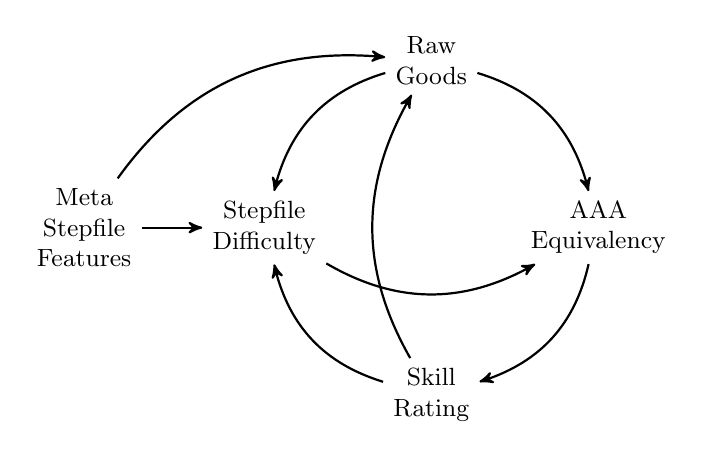
\begin{tikzpicture}[->,>=stealth',auto,align=center,node distance=3cm,
					thick,main node/.style={font=\small}]
					
					\node[main node] (1) {Meta\\Stepfile\\Features};
					\node[main node] (2) [right=1.5cm] {Stepfile\\Difficulty};
					\node[main node] (3) [below right of=2] {Skill\\Rating};
					\node[main node] (4) [above right of=2] {Raw\\Goods};
					\node[main node] (5) [above right of=3] {AAA\\Equivalency};
					
					\path[every node/.style={font=\sffamily\small}]
					(1) edge node [left] {} (2)
					(1) edge [bend left] node [right] {} (4)
					(4) edge [bend right] node [right] {} (2)
					(3) edge [bend left] node [right] {} (4)
					(4) edge [bend left] node [right] {} (5)
					(2) edge [bend right] node [right] {} (5)
					(5) edge [bend left] node [right] {} (3)
					(3) edge [bend left] node [right] {} (2);
					    
				\end{tikzpicture}
			}
		\end{subfloat}
		\hspace{10pt}       
		\begin{subfloat}[Proposed State] {
				\centering
				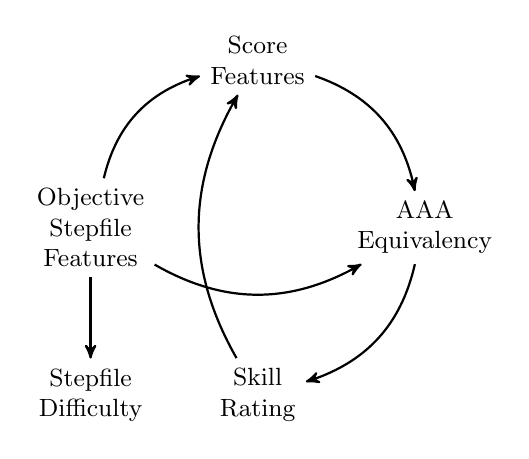
\begin{tikzpicture}[->,>=stealth',auto,align=center,node distance=3cm,
					thick,main node/.style={font=\small}]
					
					\node[main node] (1) {Stepfile\\Difficulty};
					\node[main node] (2) [above=1.5cm] {Objective\\Stepfile\\Features};
					\node[main node] (3) [below right of=2] {Skill\\Rating};
					\node[main node] (4) [above right of=2] {Score\\Features};
					\node[main node] (5) [above right of=3] {AAA\\Equivalency};
					
					\path[every node/.style={font=\sffamily\small}]
					(2) edge node [left] {} (1)
					(2) edge [bend left] node [right] {} (4)
					(3) edge [bend left] node [right] {} (4)
					(4) edge [bend left] node [right] {} (5)
					(2) edge [bend right] node [right] {} (5)
					(5) edge [bend left] node [right] {} (3);
					    
				\end{tikzpicture}
			}       
		\end{subfloat}
		\caption{Dependency graphs differentiating the current and proposed states of skill-based FFR metrics.}
		\label{fig1}
		
	\end{figure}  
\end{center}

Additionally, it is important to note that the Proposed State, as illustrated in Figure \ref{fig1}b, exhibits a circular interdependence between Score Features, AAA Equivalency, and Skill Rating. A well-designed system should be able to:

\begin{itemize}
	\item Accurately assess a player's performance on a stepfile by utilizing score features derived from a predetermined skill rating metric.
	\item Calculate AAA Equivalency without making the assumption of uniform distribution of notes within the stepfile and also take into account performance metrics that are more focused on the player.
	\item Continuously adjust a player's skill rating without distorting their true skill level, which may be influenced by factors such as the number of stepfiles played.
\end{itemize}

The implementation of this study necessitates the development of a framework for training machine learning models using the expectation-maximization algorithm. Within this framework, the models are optimized concerning their corresponding dependent skill-based metrics based on a predetermined convergence criterion. Further details on this approach will be discussed in Section [TODO], with detailed steps for the technical implementation outlined in Section [TODO].

% \vspace{2mm}

% In Section \ref{sec:stepfile_difficulty}, we aim to establish a clear definition of stepfile difficulty by addressing the inherent subjectivity of this concept. We will examine various existing interpretations and propose a methodology for estimating difficulty based on these definitions. This process includes creating a data stratification strategy to incorporate player feedback from \texttt{\#difficulty-discussion} in FFR's Official Discord channel within our train-test split, identifying a set of objectively defined features that align with specific gameplay properties, and devising a framework for training and evaluating a time series extrinsic regression model. This model will be used to replicate experiments under varying hyperparameter configurations and considered definitions.

% \vspace{2mm}

% Our definition of AAA equivalency is consistent with the interpretation of the community. However, in Section [TODO], we propose improvements to the current formula by defining an adjusted raw good count concerning features identified for our stepfile difficulty model. Additionally, we introduce precision and recall as performance-indicative metrics within the realm of competitive gameplay by defining the ``Boo" judge accuracy label as false positives and the ``Miss" judge accuracy label as false negatives.

% \vspace{2mm}

% In Section [TODO], we propose a study advocating for the incorporation of outlier detection techniques to eliminate unrepresentative AAA equivalency scores. We also present a framework for adjusting the value of $N$ depending on the number of stepfiles played. Furthermore, we suggest incorporating Seasonal Skill Ratings to contextualize players' abilities beyond their top-performing scores and evaluate their performance in comparison to Skill Ratings.

\clearpage
\section{Stepfile Difficulty Model}
\label{sec:stepfile_difficulty}

Stepfile difficulty has been a persistent subject of debate within the Flash Flash Revolution (FFR) community. Accurately defining the difficulty level of a specific sequence of keystrokes necessitates careful analysis of shared patterns across various stepfiles, which inherently exposes the process to player subjectivity. Despite attempts to leverage machine learning and artificial intelligence to address this issue, no solutions have successfully integrated the established concepts of stepfile difficulty. This limitation stems primarily from the fact that individual players possess diverse interpretations of what constitutes a difficult stepfile, shaped by their unique playing objectives and physical capabilities. Consequently, community resolutions regarding stepfile difficulty frequently result in biased judgments and disagreements. To effectively address these challenges, it is essential to standardize the definition of stepfile difficulty and to differentiate between the associated objective characteristics and the inherent subjectivity involved in such assessments.

\subsection{Playing Objective Categorizations}

\textit{Playing objectives} are goals players set to optimize in their gameplay. These playing objectives can be categorized into two main groups: constant weighted and variable weighted. This section focuses on providing numerous examples of both types of playing objectives, discussing their integration into our analysis, and establishing a default playing objective to be utilized in this report. It is imperative to acknowledge that, at present, ACubed currently supports only stepfile difficulty measurements under discretized constant weighted playing objectives. In upcoming releases, ACubed is expected to expand its capabilities to encompass additional playing objectives as we deliberate on methods to implement this in our framework.

\subsubsection{Constant-Weighted Playing Objectives}

A fundamental aspect of \textit{constant-weighted} playing objectives is the assumption that the reward for successfully hitting a note remains consistent at the note-level. Namely, each attempt at hitting a note in the stepfile receives a consistently defined reward value between $0$ and $1$, which reflects the player's incentive to successfully hit the note at some timestamp relative to the exact timing requirements for a given note. The following are examples of commonly used playing objectives falling within this category.

\begin{itemize}
    \item The Full-Combo (FC) score incentivizes players to hit all notes without missing any. The reward function to FC a stepfile is:

    $$r(t) = \begin{cases} 
          1 & -117 \leq t \leq 118 \\
          0 & \text{otherwise}
       \end{cases}$$

    \item To achieve a Clean Full-Combo score, players must hit all notes without any average hits or boo hits in addition to achieving an FC on the stepfile. The reward function to Clean FC a stepfile is:

    $$r(t) = \begin{cases} 
          1 & -83 \leq t \leq 118 \\
          0 & \text{otherwise}
       \end{cases}$$

    \item In order to maximize the score under FFR's Judge Windows, players should aim to optimize the raw score of a stepfile using the specified weights discussed in the previous section. The reward function to maximize raw score under FFR scoring is:

    $$r(t) = \begin{cases} 
          0.1 & -117 \leq t < -83 \\
          0.5 & -83 \leq t < -50 \\
          1 & -50 \leq t \leq 50 \\
          0.5 & 50 < t \leq 118 \\
          0 & \text{otherwise}
       \end{cases}$$

    \item Maximizing the score under MS Timing is not specific to FFR, but it involves optimizing the raw score of a stepfile where the assigned rewards favor hits that are closest to Perfect. This method of scoring is commonly implemented in other rhythm games, such as Etterna. The reward function to maximize raw score under MS timing is:

    $$r(t) = \begin{cases} 
          1- \frac{t}{118} & 0 \leq t \leq 118 \\
          1 + \frac{t}{117} & -117 \leq t \leq 0 \\
          0 & \text{otherwise}
       \end{cases}$$

    \item Scoring a AAA on a stepfile requires players to hit all notes within FFR's Perfect timing window. AAA is the maximum score a player can obtain on any stepfile in FFR. The reward function to score a AAA on a stepfile is:

    $$r(t) = \begin{cases} 
          1 & -50 \leq t \leq 50 \\
          0 & \text{otherwise}
       \end{cases}$$

    \item Scoring a AAAA on a stepfile requires players to hit all notes within FFR's Marvelous timing window. Despite AAAA's being significantly more difficult to obtain, these scores are treated as AAA for ranking purposes. The reward function to score a AAAA on a stepfile is:

    $$r(t) = \begin{cases} 
          1 & -17 \leq t \leq 17 \\
          0 & \text{otherwise}
       \end{cases}$$
\end{itemize}

Figure \ref{fig:playing_objectives} visually presents the various playing objectives, with the green colors denoting the reward given when a player successfully hits the correct note within the predetermined judge window.  

\begin{figure}[H]
\centering
\begin{tikzpicture}

    \begin{scope}
        \shade[top color=perfect-color, bottom color=perfect-color] (-1,-1) rectangle (4,0);
\shade[top color=perfect-color, bottom color=perfect-color] (-1,0) rectangle (4,1);
\node[inner sep=0pt] (left) at (0,0)
    {
\includegraphics[width=1cm]{figures/receptor/left.png}};
\node[inner sep=0pt] (down) at (1,0)
    {
\includegraphics[width=1cm]{figures/receptor/down.png}};
\node[inner sep=0pt] (up) at (2,0)
    {
\includegraphics[width=1cm]{figures/receptor/up.png}};
\node[inner sep=0pt] (right) at (3,0)
    {
\includegraphics[width=1cm]{figures/receptor/right.png}};
\node[inner sep=0pt] at (-1,-1)[label=left:{\footnotesize\texttt{118ms}}]{};
\draw[opacity=0.5,dashed] (-1, -1) -- (4, -1); 
\node[inner sep=0pt] at (-1,0) [label=left:{\footnotesize \texttt{0ms}}]{};
\draw[opacity=0.5,dashed] (-1, 0) -- (4, 0); 
\node[inner sep=0pt] at (-1,1) [label=left:{\footnotesize \texttt{-117ms}}]{};
\draw[opacity=0.5,dashed] (-1, 1) -- (4, 1);
\node[inner sep=0pt] at (1.5, -1.5) [label=center:{\footnotesize \textit{(a)} Full-Combo (FC)}]{};
    \end{scope}

    \begin{scope}[xshift=8cm]
\shade[top color=perfect-color, bottom color=perfect-color] (-1,-1) rectangle (4,0);
\shade[top color=perfect-color, bottom color=perfect-color] (-1,0) rectangle (4,0.083/0.118);
\node[inner sep=0pt] (left) at (0,0)
    {
\includegraphics[width=1cm]{figures/receptor/left.png}};
\node[inner sep=0pt] (down) at (1,0)
    {
\includegraphics[width=1cm]{figures/receptor/down.png}};
\node[inner sep=0pt] (up) at (2,0)
    {
\includegraphics[width=1cm]{figures/receptor/up.png}};
\node[inner sep=0pt] (right) at (3,0)
    {
\includegraphics[width=1cm]{figures/receptor/right.png}};
\node[inner sep=0pt] at (-1,-1)[label=left:{\footnotesize\texttt{118ms}}]{};
\draw[opacity=0.5,dashed] (-1, -1) -- (4, -1); 
\node[inner sep=0pt] at (-1,0) [label=left:{\footnotesize \texttt{0ms}}]{};
\draw[opacity=0.5,dashed] (-1, 0) -- (4, 0); 
\node[inner sep=0pt] at (-1,1) [label=left:{\footnotesize \texttt{-117ms}}]{};
\draw[opacity=0.5,dashed] (-1, 1) -- (4, 1);
\node[inner sep=0pt] at (1.5, -1.5) [label=center:{\footnotesize \textit{(b)} Clean Full-Combo (FC)}]{};
    \end{scope}

    \begin{scope}[yshift=-3.5cm]
        \shade[top color=perfect-color, bottom color=perfect-color, opacity=0.5] (-1,-1) rectangle (4,-0.050/0.117);
\shade[top color=perfect-color, bottom color=perfect-color] (-1,-0.050/0.117) rectangle (4,0);
\shade[top color=perfect-color, bottom color=perfect-color] (-1,0) rectangle (4,0.050/0.118);
\shade[top color=perfect-color, bottom color=perfect-color, opacity=0.5] (-1,0.050/0.118) rectangle (4,0.083/0.118);
\shade[top color=perfect-color, bottom color=perfect-color, opacity=0.1] (-1,0.083/0.118) rectangle (4,1);
\node[inner sep=0pt] (left) at (0,0)
    {
\includegraphics[width=1cm]{figures/receptor/left.png}};
\node[inner sep=0pt] (down) at (1,0)
    {
\includegraphics[width=1cm]{figures/receptor/down.png}};
\node[inner sep=0pt] (up) at (2,0)
    {
\includegraphics[width=1cm]{figures/receptor/up.png}};
\node[inner sep=0pt] (right) at (3,0)
    {
\includegraphics[width=1cm]{figures/receptor/right.png}};
\node[inner sep=0pt] at (-1,-1)[label=left:{\footnotesize\texttt{118ms}}]{};
\draw[opacity=0.5,dashed] (-1, -1) -- (4, -1); 
\node[inner sep=0pt] at (-1,0) [label=left:{\footnotesize \texttt{0ms}}]{};
\draw[opacity=0.5,dashed] (-1, 0) -- (4, 0); 
\node[inner sep=0pt] at (-1,1) [label=left:{\footnotesize \texttt{-117ms}}]{};
\draw[opacity=0.5,dashed] (-1, 1) -- (4, 1);
\node[inner sep=0pt] at (1.5, -1.5) [label=center:{\footnotesize \textit{(c)} Maximize Score under FFR Scoring (Default)}]{};
    \end{scope}

    \begin{scope}[xshift=8cm, yshift=-3.5cm]
\shade[top color=perfect-color, bottom color=white] (-1,-1) rectangle (4,0);
\shade[top color=white, bottom color=perfect-color] (-1,0) rectangle (4,1);
\node[inner sep=0pt] (left) at (0,0)
    {
\includegraphics[width=1cm]{figures/receptor/left.png}};
\node[inner sep=0pt] (down) at (1,0)
    {
\includegraphics[width=1cm]{figures/receptor/down.png}};
\node[inner sep=0pt] (up) at (2,0)
    {
\includegraphics[width=1cm]{figures/receptor/up.png}};
\node[inner sep=0pt] (right) at (3,0)
    {
\includegraphics[width=1cm]{figures/receptor/right.png}};
\node[inner sep=0pt] at (-1,-1)[label=left:{\footnotesize\texttt{118ms}}]{};
\draw[opacity=0.5,dashed] (-1, -1) -- (4, -1); 
\node[inner sep=0pt] at (-1,0) [label=left:{\footnotesize\texttt{0ms}}]{};
\draw[opacity=0.5,dashed] (-1, 0) -- (4, 0); 
\node[inner sep=0pt] at (-1,1) [label=left:{\footnotesize\texttt{-117ms}}]{};
\draw[opacity=0.5,dashed] (-1, 1) -- (4, 1);
\node[inner sep=0pt] at (1.5, -1.5) [label=center:{\footnotesize \textit{(d)} Maximize Score under MS-based Timings}]{};
    \end{scope}

    \begin{scope}[yshift=-7cm]
\shade[top color=perfect-color, bottom color=perfect-color] (-1,-0.050/0.117) rectangle (4,0.050/0.118);
\node[inner sep=0pt] (left) at (0,0)
    {
\includegraphics[width=1cm]{figures/receptor/left.png}};
\node[inner sep=0pt] (down) at (1,0)
    {
\includegraphics[width=1cm]{figures/receptor/down.png}};
\node[inner sep=0pt] (up) at (2,0)
    {
\includegraphics[width=1cm]{figures/receptor/up.png}};
\node[inner sep=0pt] (right) at (3,0)
    {
\includegraphics[width=1cm]{figures/receptor/right.png}};
\node[inner sep=0pt] at (-1,-1)[label=left:{\footnotesize\texttt{118ms}}]{};
\draw[opacity=0.5,dashed] (-1, -1) -- (4, -1); 
\node[inner sep=0pt] at (-1,0) [label=left:{\footnotesize \texttt{0ms}}]{};
\draw[opacity=0.5,dashed] (-1, 0) -- (4, 0); 
\node[inner sep=0pt] at (-1,1) [label=left:{\footnotesize \texttt{-117ms}}]{};
\draw[opacity=0.5,dashed] (-1, 1) -- (4, 1);
\node[inner sep=0pt] at (1.5, -1.5) [label=center:{\footnotesize \textit{(e)} All Perfects (AAA)}]{};
    \end{scope}

    \begin{scope}[xshift=8cm, yshift=-7cm]
\shade[top color=perfect-color, bottom color=perfect-color] (-1,-0.017/0.117) rectangle (4,0.017/0.118);
\node[inner sep=0pt] (left) at (0,0)
    {
\includegraphics[width=1cm]{figures/receptor/left.png}};
\node[inner sep=0pt] (down) at (1,0)
    {
\includegraphics[width=1cm]{figures/receptor/down.png}};
\node[inner sep=0pt] (up) at (2,0)
    {
\includegraphics[width=1cm]{figures/receptor/up.png}};
\node[inner sep=0pt] (right) at (3,0)
    {
\includegraphics[width=1cm]{figures/receptor/right.png}};
\node[inner sep=0pt] at (-1,-1)[label=left:{\footnotesize\texttt{118ms}}]{};
\draw[opacity=0.5,dashed] (-1, -1) -- (4, -1); 
\node[inner sep=0pt] at (-1,0) [label=left:{\footnotesize \texttt{0ms}}]{};
\draw[opacity=0.5,dashed] (-1, 0) -- (4, 0); 
\node[inner sep=0pt] at (-1,1) [label=left:{\footnotesize \texttt{-117ms}}]{};
\draw[opacity=0.5,dashed] (-1, 1) -- (4, 1);
\node[inner sep=0pt] at (1.5, -1.5) [label=center:{\footnotesize \textit{(f)} All Marvelous (AAAA)}]{};
    \end{scope}

\end{tikzpicture}

\caption{Constant-Weighted Playing Objectives to define Stepfile Difficulty.} \label{fig:playing_objectives}
\end{figure}

It is worth mentioning that since the manually assigned difficulty ratings are determined under the goal of achieving the highest possible raw score with FFR judgement windows, our definition of the stepfile difficulty model will be aligned with this particular playing objective. Additional manual data collection is necessary to develop a stepfile difficulty model that can support other playing objectives identified in this report.

\vspace{2mm}

To allow for meaningful comparisons, each playing objective can be represented by an equivalent judge window size $J$. This can be determined by evaluating the following integral:

$$J = \displaystyle \int_{-\infty}^{\infty} r(t) dt$$

For example, for score maximizing playing objectives under FFR judgement windows, we have:
\begin{align*}
J &= \displaystyle \int_{-\infty}^{\infty} r(t) dt \\
& = 0.1 \cdot (-83 - (-117)) + 0.5 \cdot (-50 - (-83)) + 1 \cdot (50 - (-50)) + 0.5 \cdot (118 - 50) \\
&= 3.4 + 16.5 + 100 + 34 = 153.9
\end{align*}

and for score maximizing playing objectives under MS Timing, we have:
\begin{align*}
J &= \displaystyle \int_{-\infty}^{\infty} r(t) dt \\
& = \int_{0}^{118} \left(1 - \frac{t}{118}\right) dt + \int_{-117}^{0} \left(1 + \frac{t}{117}\right) dt \\
&= \left. \left( t - \frac{t^2}{236} \right)\right|_{t = 118} - \left.\left( t + \frac{t^2}{234} \right) \right|_{t = - 117} \\
&= 59 + 58.5 = 117.5
\end{align*}

Moreover, with the assumption that the weight values for Etterna's Perfect, Great, and Good ratings are $1$, $0.5$, and $0.1$ respectively, \href{https://docs.google.com/spreadsheets/d/1syi5aN6sTiDA2Bs_lzZjsLQ1yCEhxl5EnAd6EsD6cF4/edit?gid=0#gid=0}{Etterna Judgement Data} was incorporated into the analysis for comparison. Through similar calculations, it was determined that the corresponding equivalent judge window sizes for each identified playing objective are as follows:

\begin{center}
	\begin{tabular}{c@{\hskip 5mm}c}
		\hspace{5mm} \textbf{Playing Objective} \hspace{5mm} & \textbf{Equivalent Window Size} $J$ \\
            \hline
		Full-Combo in FFR                              & 235                        \\
            Maximize Score in Etterna Under J1 & 216\\
		Clean Full-Combo in FFR                                 & 201                         \\
            Maximize Score in Etterna Under J2 & 191.52\\
            Maximize Score in Etterna Under J3 & 167.04\\
		Maximize Score in FFR assuming default scoring                              & 153.9                       \\
            Maximize Score in Etterna Under J4 & 144\\
            Maximize Score in Etterna Under J5 & 120.96\\
		Maximize Score in FFR assuming MS-weighted scoring                                  & 117.5                       \\
  
		Scoring AAA in FFR                                   & 100                    \\
            Maximize Score in Etterna Under J6 & 95.04\\
            Maximize Score in Etterna Under J7 & 72\\
            Maximize Score in Etterna Under J8 & 47.52\\
		Scoring AAAA in FFR                                   & 34                       \\
            Maximize Score in Etterna Under J9 & 28.8\\
	\end{tabular}
\end{center}

The execution of the playing objective is more challenging when $J$ values are lower, as indicated by a smaller judge window which allows for a narrower margin of error. This examination corroborates the general perception within the community that the FFR's scoring system falls between Etterna's J3 and J4 scoring, with the latter being known as Etterna's default judgement setting. 

\vspace{2mm}

These computed judge windows will be utilized in this report to enhance the definition of objective features that are employed in the stepfile difficulty model. Further details on integrating judge window size to the objective features associated to the stepfile difficulty model will be discussed later in this section.

\subsubsection{Variable-Weighted Playing Objectives}

The concept of variable-weighted playing objectives posits that the reward attributed to each note can vary depending on the player's previous actions. This means that the reward value, which similarly ranges from 0 to 1, does not necessarily require a perfect hit for every note to fulfill the playing objective. The following playing objectives are categorized as variable-weighted:

\begin{itemize}
    \item The utilization of atypical playing tactics for the purpose of generating non-conventional scores is a fundamental aspect of the Anti-PA scoring methodology. This strategic approach is typically employed by players in order to unlock \href{https://www.flashflashrevolution.com/tokens/skill_token_info.php}{skill tokens in FFR}.

    \item In order to obtain a Single-Digit Good (SDG) score, players must achieve a score of less than ten raw goods on a stepfile. SDG is commonly recognized by players as a crucial milestone in their pursuit of achieving a AAA score on that particular stepfile.
\end{itemize}



It is worth noting that the aforementioned examples can be generalized as scoring-based objectives, in which the player's aim is to reach a predetermined score. However, depending on the miss and boo requirements of the targeted score, the player must additionally manage the life bar when gameplay is in session. Shown on the right of Figure \ref{fig:gameplay}, the life bar represents a player's remaining life during gameplay. Each successful hit on an arrow contributes to increasing the bar, whereas receiving a Miss or Boo judgement will result in a decrease. Allowing the bar to deplete entirely will result in the conclusion of the game.

\begin{center}
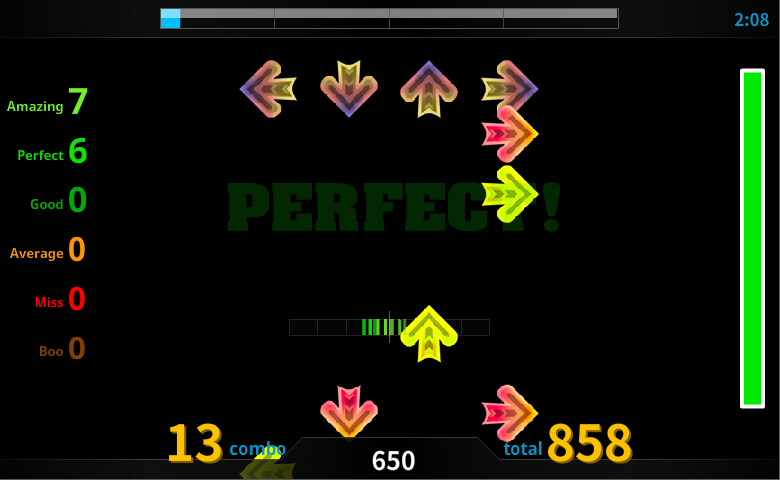
\includegraphics[width=10cm]{figures/images/gameplay.png}
\captionof{figure}{Screenshot of FFR's Gameplay View (upscroll view)}
\label{fig:gameplay}
\end{center}

While the addition of the life bar in gameplay introduces implementation challenges in measuring the difficulty of these playing objectives, we offer potential solutions for addressing this issue. We commence by positing a theorem and reinforcing it with a heuristic demonstration.

\begin{theorem}
\label{thm:finiteness}
Given any targeted score under the variable-weighted playing objective, there are finitely many ways for a player to accomplish this. 
\end{theorem}

\begin{proof}
    Let $B$ represent the number of boos in the targeted score and let $N$ represent the number of notes in the stepfile. As boos can only appear between two notes, we can count the number of ways to assort $B$ boos with $N$ notes using stars and bars. Let $\times$ represent boos and $\mid$ represent notes, and arrange the objects sequentially as shown in Figure \ref{fig:starsandbars1}.

\vspace{2mm}

\begin{center}
$ \times \mid\times\mid \; \mid \times \times \mid \; \mid \; \mid \times$
\captionof{figure}{An example of Stars and Bars for $N=6$ notes and $B =5$ boos}
\label{fig:starsandbars1}
\end{center}

Because there are a total of $N+B$ objects, there are $\displaystyle \binom{N+B}{B}$ ways to arrange $N$ notes and $B$ boos.

\vspace{2mm}

Furthermore, let $H$ represent the number of successfully hit notes and $M$ represent the number of missed notes. Observe that $H + M = N$. Using the previously discussed Stars and Bars analogy, if we let $+$ and $-$ represent hits and misses respectively while ignoring the $\times$, we can replace each $\mid$ with these symbols as shown in Figure \ref{fig:starsandbars2}.

\vspace{2mm}

Per arrangement from the first iteration of Stars and Bars, there are $\displaystyle\binom{H + M}{M}$ ways to arrange $H$ hits and $M$ misses.

\begin{center}
$ \times \mid\times\mid \; \mid \times \times \mid \; \mid \; \mid \times$ 	\hspace{5mm} $\Longrightarrow$ \hspace{5mm} $\times + \times +  - \times \times ++- \times $
\captionof{figure}{Replacing $N=6$ notes with $H=4$ hits and $M = 2$ misses}
\label{fig:starsandbars2}
\end{center}

We apply the same argument to conclude that the number of ways to arrange $P$ perfects, $G$ goods, and $A$ averages over $H = P + G + A$ hits is:
$$\displaystyle \binom{P + G + A}{A}\binom{P+G}{G}$$

Combining everything together, the number of possible ways a player can score $P$ perfects, $G$ goods, $A$ averages, $M$ misses, and $B$ boos in a stepfile containing $N$ notes, regardless of the life bar's status, is:
$$\displaystyle \binom{P+G+A+M+B}{B}\binom{P+G+A+M}{M} \binom{P + G + A}{A}\binom{P+G}{G} = \binom{N+B}{P, G, A, M, B}.$$

We can obtain sharper upper bounds when we consider the status of the life bar in our overall counts. Using the same variable definitions, let $J$ represent the number of ``no-hit" actions (i.e. $J = M + B$). Then, our combinatorics problem can be reformulated as:
$$j_1 + j_2 + \cdots + j_{H + 1} = H + J$$

where $j_i$ represents the number of ``no-hit" actions in the $i$th bin (i.e. number of misses and boos between the $(i-1)$th and $i$th hits). Applying Stars and Bars without any constraints, the number of integer solutions to the above problem is $\displaystyle \binom{H+J}{H}$.

\vspace{2mm}

As the maximum health in the life bar is $20$, then for all $j_i$, we have $j_i \leq 20$. To enforce the constraint for $k$ $j_i$'s, we need to exclude all solutions with $j_{i_1} > 20$, $j_{i_2} > 20$, $\cdots$, $j_{i_k} > 20$ for $0 \leq i_1 \neq i_2 \neq \cdots \neq i_k \leq \left\lfloor\frac{J}{21} \right\rfloor$ (to ensure that $J - 21k \geq 0$). The above problem under these constraints can be reformulated as:
$$j_1 + \cdots + (j_{i_1} - 21) + (j_{i_2} - 21) + \cdots + (j_{i_k} - 21) 
+ \cdots + j_{H + 1} = H + J - 21k.$$

There are $\displaystyle \binom{H+1}{k}$ ways to choose the $k$ $j_i$'s and for each $k$, there are $\displaystyle\binom{H+J-21k}{H}$ solutions.

\vspace{2mm}

By applying the Inclusion–Exclusion principle across all $k-$tuples of $j_i$'s satisfying the above constraint, we get:
$$\sum_{k =0}^{\left\lfloor \frac{J}{21}\right\rfloor} (-1)^k \binom{H + 1}{k}\binom{H+J-21k}{H}.$$

Therefore, the number of possible ways a player can score $P$ perfects, $G$ goods, $A$ averages, $M$ misses, and $B$ boos in a stepfile containing $N$ notes is:
$$\sum_{k =0}^{\left\lfloor \frac{M+B}{21}\right\rfloor} (-1)^k \binom{P+G+A + 1}{k}\binom{N+B-21k}{P+G+A}.$$

We claim that this count is an upper bound to the total number of ways a player can actually produce such scores in actual gameplay. This is due to the fact that the count accounts for scenarios where $j_1 \geq 10$ (indicating that the number of misses and boos before hitting the first note is greater than or equal to $10$) is not deemed a failure, when in reality it would result in the conclusion of the game. 

\end{proof}

Let $f$ represent the stepfile difficulty model that maps the set of all input configurations that result in a predetermined desired score $\mathcal{C}_{\text{score}}$ to a positive real number. Hence, following the establishment of finiteness through Theorem \ref{thm:finiteness}, it can be deduced that there exists an input configuration such that $f$ is minimal. This particular configuration can be considered as the most optimal way for a player to achieve the desired score.

\vspace{2mm}

It is assumed that if a player is able to achieve a higher-rated input configuration, then they are also capable of achieving the optimal configuration. Under this assumption, we rate the stepfile difficulty under variable-weighted playing objectives by evaluating the following optimization problem:

\begin{equation*}
\begin{aligned}
\min_{c \in \mathcal{C}_{\text{score}}} \quad & f(c)\\
\textrm{s.t.} \quad & \text{score} = (P, G, A, M, B)  
\end{aligned}
\end{equation*}

Currently, the exact criteria for determining the judge window size in variable-weighted playing objectives has yet to be established. Without loss of generality, consider all notes in a given stepfile that are oriented upwards. We will refer to the example shown in Figure \ref{fig:boos} for context.

\begin{center}
\begin{tikzpicture}
        \shade[top color=perfect-color, bottom color=perfect-color, opacity=0.5] (-1,-1 +2.5+1.25) rectangle (4,-0.050/0.117 +2.5+1.25);
\shade[top color=perfect-color, bottom color=perfect-color] (-1,-0.050/0.117 +2.5+1.25) rectangle (4,0.050/0.118 +2.5+1.25);
\shade[top color=perfect-color, bottom color=perfect-color, opacity=0.5] (-1,0.050/0.118 +2.5+1.25) rectangle (4,0.083/0.118 +2.5+1.25);
\shade[top color=perfect-color, bottom color=perfect-color, opacity=0.1] (-1,0.083/0.118 +2.5+1.25) rectangle (4,1 +2.5+1.25);
\node[inner sep=0pt] (up) at (2,0 +2.5+1.25)
    {
\includegraphics[width=1cm]{figures/016/up.png}};



        \shade[top color=perfect-color, bottom color=perfect-color, opacity=0.5] (-1,-1 +2.5) rectangle (4,-0.050/0.117 +2.5);
\shade[top color=perfect-color, bottom color=perfect-color] (-1,-0.050/0.117 +2.5) rectangle (4,0.050/0.118 +2.5);
\shade[top color=perfect-color, bottom color=perfect-color, opacity=0.5] (-1,0.050/0.118 +2.5) rectangle (4,0.083/0.118 +2.5);
\shade[top color=perfect-color, bottom color=perfect-color, opacity=0.1] (-1,0.083/0.118 +2.5) rectangle (4,1 +2.5);
\node[inner sep=0pt] (up) at (2,0 +2.5)
    {
\includegraphics[width=1cm]{figures/008/up.png}};
        
        \shade[top color=perfect-color, bottom color=perfect-color, opacity=0.5] (-1,-1) rectangle (4,-0.050/0.117);
\shade[top color=perfect-color, bottom color=perfect-color] (-1,-0.050/0.117) rectangle (4,0.050/0.118);
\shade[top color=perfect-color, bottom color=perfect-color, opacity=0.5] (-1,0.050/0.118) rectangle (4,0.083/0.118);
\shade[top color=perfect-color, bottom color=perfect-color, opacity=0.1] (-1,0.083/0.118) rectangle (4,1);
\node[inner sep=0pt] (up) at (2,0)
    {
\includegraphics[width=1cm]{figures/004/up.png}};

\node[inner sep=0pt] (left) at (0,-1.75)
    {
\includegraphics[width=1cm]{figures/receptor/left.png}};
\node[inner sep=0pt] (down) at (1,-1.75)
    {
\includegraphics[width=1cm]{figures/receptor/down.png}};
\node[inner sep=0pt] (up) at (2,-1.75)
    {
\includegraphics[width=1cm]{figures/receptor/up.png}};
\node[inner sep=0pt] (right) at (3,-1.75)
    {
\includegraphics[width=1cm]{figures/receptor/right.png}};

\draw[opacity=0.5,dashed] (-1, 2.5+0.625) -- (4, 2.5+0.625); 
\node[inner sep=0pt] at (-1,2.5+0.625) [label=left:{\footnotesize $b_2$}]{};
\node[inner sep=0pt] (up) at (2,2.5+0.625)
    {$\textcolor{orange}{\boldsymbol{\times}}$};
\node[inner sep=0pt] (up) at (2,2.5+0.625+0.01)
    {$\textcolor{orange}{\boldsymbol{\times}}$};
\node[inner sep=0pt] (up) at (2,2.5+0.625-0.01)
    {$\textcolor{orange}{\boldsymbol{\times}}$};
\node[inner sep=0pt] (up) at (2+0.01,2.5+0.625)
    {$\textcolor{orange}{\boldsymbol{\times}}$};
\node[inner sep=0pt] (up) at (2-0.01,2.5+0.625)
    {$\textcolor{orange}{\boldsymbol{\times}}$};

\draw[opacity=0.5,dashed] (-1, 1.25) -- (4, 1.25); 
\node[inner sep=0pt] at (-1,1.25) [label=left:{\footnotesize $b_1$}]{};
\node[inner sep=0pt] (up) at (2,1.25)
    {$\textcolor{orange}{\boldsymbol{\times}}$};
\node[inner sep=0pt] (up) at (2,1.25+0.01)
    {$\textcolor{orange}{\boldsymbol{\times}}$};
\node[inner sep=0pt] (up) at (2,1.25-0.01)
    {$\textcolor{orange}{\boldsymbol{\times}}$};
\node[inner sep=0pt] (up) at (2+0.01,1.25)
    {$\textcolor{orange}{\boldsymbol{\times}}$};
\node[inner sep=0pt] (up) at (2-0.01,1.25)
    {$\textcolor{orange}{\boldsymbol{\times}}$};

\end{tikzpicture}
\captionof{figure}{Incorporating Boos in Judge Window Size computation}
\label{fig:boos}
\end{center}

In the event that a player taps the keyboard at timestamp $b_1$ between the red and blue notes, the engine will record a Boo towards the final score. This is due to the fact that the judge windows for these notes do not overlap, allowing the possibility for the player to hit a Boo. The corresponding judge window size for successfully hitting this Boo is visually represented by the white-colored distance between the two judgment windows.

\vspace{2mm}

Conversely, if a player submits input at timestamp $b_2$ between the blue and yellow notes, the engine will record an early good in the judge window of the yellow note if the blue note was not previously hit, or a late good in the blue note's judge window if it was successfully hit. Given that these windows overlap, there is no opportunity for the player to hit a Boo, resulting in a judge window size of $0$ for this instance.

\vspace{2mm}

In terms of misses, as no action is required on the player's behalf, no judge window sizes are factored in the calculation of the overall difficulty of the stepfile under this playing objective. Essentially, misses can be disregarded as the domain space of all possible configurations assumes that the player will not fail the level.

\vspace{2mm}

Due to the fact that all variable-weighted playing objectives solely focus on players hitting a certain number of notes with different judgments, rather than specifying the exact timing of when to hit them, the evaluation of stepfile difficulty can be determined by finding the optimal configuration that increases the likelihood of achieving the desired judgments. This involves identifying the optimum judge window sizes and computing the overall weighted average once the configuration has been identified.

\subsection{Machine Learning Problem Formulation}

With a clear distinction made between different interpretations of difficulty, our focus now shifts to formulating the measurement of stepfile difficulty as a machine learning problem using the chosen definition as the de facto standard. In this section, we will define key terms and present a theorem as the basis for our methodology.

\vspace{2mm}

Stepfile features have a significant impact on identifying the factors that contribute to the level's difficulty. Thus, it is essential to utilize these features in constructing a predictive model for estimating stepfile difficulty. These features fall under two distinct categories, namely, objective and subjective.

\begin{itemize}
    \item \textit{Objective stepfile features} refer to characteristics of a stepfile that contain rigid requirements independent of the player's skill level. These may include precise timing requirements for all arrows and the duration of the stepfile. Note that meta stepfile features are not considered objective, as the established definition to differentiate patterns from one another cannot be codified deterministically. 
    \item \textit{Subjective stepfile features} are defined as elements that are primarily centered on the execution of the stepfile and are subject to the player's individual skill level. These features may include factors related to a player's ability to execute the steps accurately, as well as their access to high-quality equipment. For instance, a player with greater stamina is likely to excel at longer stepfiles and may tend to underestimate its level of challenge as a result. 
\end{itemize}

Using these stepfile features, we propose the following theorem.

\begin{theorem}
Given a stepfile, the true difficulty rating can be estimated with a machine learning model using the objective stepfile features and the upper echelons of player telemetry.
\end{theorem}

\begin{proof}

Consider a scenario where there are $n$ players, denoted as $A_1, A_2,\ldots,A_n$, tasked with providing feedback on the difficulty of a given stepfile. Each player, $A_i$ for all $1 \leq i \leq n$, relies on the stepfile's distinct attributes and their own personal abilities to justify their assessment. Assuming that the difficulty of the stepfile is additive, we can represent this as the following equation:
$$\text{Diff}_{\text{obs}}^{(A_i)} = \text{Diff}_{\text{obj}}^{(A_i)} + \text{Diff}_{\text{sub}}^{(A_i)}.$$

Because each player $A_1, A_2, \cdots, A_n$ are exposed to the same step layout in a given stepfile, their unbiased assessments of difficulty are mutually shared. This can be mathematically expressed as follows:
$$\text{Diff}_{\text{obj}} \coloneq \text{Diff}_{\text{obj}}^{(A_1)} = \text{Diff}_{\text{obj}}^{(A_2)} = \cdots = \text{Diff}_{\text{obj}}^{(A_n)}.$$

Let $A = (A_1, \cdots, A_n)$ denote a community of $n$ players. By aggregating the individual difficulty assessments of all $n$ players, we can calculate the observed difficulty rating of a stepfile, taking into consideration the potential impact of community bias. By further refining the aforementioned equation, we arrive at the following equation:
$$\text{Diff}_{\text{obs}}^{(A)} = \text{Diff}_{\text{obj}} + \text{Diff}_{\text{sub}}^{(A)}.$$

In theory, by obtaining feedback from the entire population regarding the difficulty of a stepfile, with an unlimited sample (i.e. $n \rightarrow \infty$), it may be possible to establish an accurate measurement of difficulty that considers human limitations and reduces the influence of player subjectivity. Therefore, 
$$\lim_{n \rightarrow \infty} \text{Diff}_{\text{obs}}^{(A)} = \text{Diff}_{\text{true}}\mspace{50mu} \text{and} \mspace{50mu} \lim_{n \rightarrow \infty} \text{Diff}_{\text{sub}}^{(A)} = \text{Diff}_{\text{human}}$$

for some unknown constant $\text{Diff}_{\text{human}}$. Based on the aforementioned asymptotic analysis, it can be deduced that
$$\text{Diff}_{\text{true}} = \text{Diff}_{\text{obj}} + \text{Diff}_{\text{human}}.$$
\end{proof}

It should be noted that the current difficulty ratings in the game are represented by $\text{Diff}_{\text{obs}}^{(A)}$ in the preceding proof. Based on this, we introduce the following corollary:

\begin{corollary}
The discrepancy between the true difference $\text{Diff}_{\text{true}}$ and the observed difference $\text{Diff}_{\text{obs}}^{(A)}$ is significantly influenced by the subjective characteristics of the stepfile as defined by the vocal community. In other words,
$$|\text{Diff}_{\text{obs}}^{(A)} - \text{Diff}_{\text{true}}| = |\text{Diff}_{\text{sub}}^{(A)} - \text{Diff}_{\text{human}}|$$
\end{corollary}

In order to ensure the credibility of the given target values, it is crucial to minimize the deviation between $\text{Diff}_{\text{obs}}^{(A)}$ and $\text{Diff}_{\text{true}}$. From the above corollary, this can be accomplished by utilizing community feedback to estimate $\text{Diff}_{\text{human}}$, the role which difficulty consultants play when receiving new opinions from community members. This requires us to gather more feedback from the community, which is highly susceptible to self-selection bias and group attribution error.

\vspace{2mm}

Instead of attempting to correct data labeling errors, we will use the ratings as targets in our supervised learning problem to estimate the true difficulty $\text{Diff}_{\text{true}}$ by maximizing the explained variation of the objective stepfile features. Doing so enables us to rely less on our inability to control identified biases in our analysis, while creating future opportunities to improve the definition of true difficulty through continued research on player telemetry and improved feature engineering from available stepfile data.
\vspace{2mm} 

We will conclude this section by presenting a formal treatment of the supervised learning problem as applied to the prediction of stepfile difficulty. Let $f: (X_{\text{obj}}^1, \cdots, X_{\text{obj}}^n) \mapsto \text{Diff}_{\text{true}}$ represent an unknown stepfile difficulty prediction model such that:
$$\text{Diff}_{\text{true}} = f(X_{\text{obj}}^1, \cdots, X_{\text{obj}}^n) + \epsilon$$

where $\epsilon$ is a random error term with mean $0$ and independent of all $X_{\text{obj}}^i$. \cite{james2023introduction} This error term is designed to capture the explained variation of features associated to player telemetry. Let $\hat{f}$ represent an estimated version of $f$ that produces the prediction $\hat{\text{Diff}_{\text{true}}} = \hat{f}(X_{\text{obj}}^1, \cdots, X_{\text{obj}}^n)$. Assuming that both $\hat{f}$ and all objective stepfile features are fixed, we have:
\begin{align*}
    E(\text{Diff}_{\text{true}} - \hat{\text{Diff}_{\text{true}}})^2 & = E(f(X_{\text{obj}}^1, \cdots, X_{\text{obj}}^n) + \epsilon - \hat{f}(X_{\text{obj}}^1, \cdots, X_{\text{obj}}^n))^2 \\
    & = [f(X_{\text{obj}}^1, \cdots, X_{\text{obj}}^n) - \hat{f}(X_{\text{obj}}^1, \cdots, X_{\text{obj}}^n)]^2 + \text{Var}(\epsilon)
\end{align*}

Similar to typical supervised learning problems, our main objective is to accurately estimate the function $f$, while also minimizing the reducible error $[f(X_{\text{obj}}^1, \cdots, X_{\text{obj}}^n) - \hat{f}(X_{\text{obj}}^1, \cdots, X_{\text{obj}}^n)]^2$. It should be noted that the stepfile features used in the supervised learning framework will be properly identified in a later section of this report.

% In addition to issues mentioned earlier in this report, the evolution of FFR's stepfile difficulty measurement demonstrates the varying perspectives on what constitutes a challenging stepfile. A notable factor contributing to this lack of a consensus is the absence of standardized criteria for determining difficulty. This section aims to establish such standards in order to establish a more reliable and trusted model for evaluating stepfile difficulty, by examining the Contested Difficulties spreadsheet and identifying the difficulty values that hold the most consensus within the FFR community.

\subsection{Modifications to Train-Test Split Methodology}

In the previous section, we formulated the machine learning problem under supervised learning using the critical assumption that all target values are labeled correctly. Although there may be inaccuracies in our predictions due to aforementioned labeling errors from the previous section, we can minimize the severity of this issue by appropriately modifying our train-test split methodology.
\vspace{2mm}

Before delving into the specifics, it is necessary to review the rationale for creating separate training and test datasets for model evaluation. In many machine learning contexts, developers often employ curve fitting techniques to identify a function that minimizes discrepancies between the model's predictions and the actual target values. However, such strategies can lead to overfitting, where the model captures not only the underlying pattern but also the noise in the training data, thereby compromising its ability to generalize to unseen data points.

\vspace{2mm}
This phenomenon underscores the importance of addressing the bias-variance tradeoff, wherein a balance is sought between a model's capacity to fit the training data and its potential to generalize to new inputs. To mitigate overfitting and evaluate a model’s generalization capability, it is standard practice in supervised learning to partition the dataset into distinct training and test sets. Typically, the test set constitutes 20\% of the entire data, while the remaining 80\% is allocated for training. Such a division ensures that the model's performance can be evaluated on an independent subset, thereby providing a more robust estimate of its predictive accuracy.

\vspace{2mm}

As the sole purpose of the test set is to assess the model's performance, it is customary to create a separate validation set for optimizing the model’s hyperparameters. The size of the validation set is typically comparable to that of the test set. This additional set allows for fine-tuning hyperparameters without compromising the independence of the test set, which remains reserved for final evaluation. Given that the success of the model in this context will be judged based on its ability to predict the difficulty of new stepfiles in FFR, we incorporate sample weights derived from known difficulty ratings. This weighting ensures that both the validation and test sets accurately reflect the community's perception of difficulty, thereby enabling more nuanced evaluations.

\vspace{2mm}

To implement this, it is crucial to identify the most pertinent data sources that align with the community's perception of stepfile difficulty. This alignment ensures that the model’s predictions can be effectively validated against community feedback and expectations.

\vspace{2mm}
One such key data source is the \href{https://docs.google.com/spreadsheets/d/1Wm1RHG318EK07U4VDXkztKTKnfy9wEOQqWRiTclbCz8/edit?gid=0#gid=0}{Contested Difficulty Spreadsheet}, managed by \texttt{Zlyice}. This collaborative Google Sheets document tracks proposed changes to stepfile difficulty measurements based on community input. Each entry in the spreadsheet reflects a suggested difficulty adjustment, operating under the assumption that contributors possess a certain degree of expertise regarding the technical and subjective factors that justify such ratings. While it is important to recognize that all proposed measurements are subject to volunteer bias, leveraging these crowd-sourced evaluations helps mitigate the influence of individual biases on any given stepfile.

\vspace{2mm}
By aggregating multiple perspectives, the community-driven approach provides a more balanced representation of perceived difficulty, which can be particularly valuable when establishing a consensus on appropriate difficulty levels. This process of integrating user feedback ensures that the resulting difficulty ratings are more reflective of the collective view, thereby enhancing the reliability of the dataset used for model evaluation and development.

\vspace{2mm}


To align our model scoring with the prevailing consensus on the quantification of stepfile difficulty within the community, we conduct a comprehensive analysis of proposed difficulty levels over the period spanning from 2022 to the present date. This analysis allows us to capture temporal trends and shifts in difficulty perceptions, ensuring that our data partitioning strategy accurately reflects current community standards. The resulting insights form the foundation of our train-test split strategy, where the distribution of proposed difficulties informs the allocation of data into appropriately representative training, validation, and test sets. By utilizing this distribution-based approach, we ensure that each dataset subset maintains a balance consistent with the overall trend of proposed difficulties, which is critical for achieving robust model performance and reliable generalization to new stepfiles.


\vspace{2mm}


\textbf{Plan:}
\begin{itemize}
	      	      
	      \item{Introduce Contested Difficulty Sheet and define train-test split using KDE estimations of proposed difficulties}
	      	      
	      \item{Introduce objective features VerticalDensity and HorizontalDensity using pen-tapping as an example. Also mention chart augmentation considerations:}
	      \begin{itemize}
	      	\item Mirror: Indirectly accounted in VerticalDensity's definition
	      	\item Offset: Indirectly accounted in preprocessing of FFR's API response.
	      	\item Colors: Categorized under "processing difficulty"; users can alter this.
	      	\item Scroll Speed Mod: Categorized under "processing difficulty"; users can alter this.
	      \end{itemize}
	      	      
	\item Dissociate local features from global features. Song length is a global feature, subsequence extraction is a local feature. Mention how ensembling works with the consideration of "difficulty spikes" in many charts.
	      	      
	\item Introduce model architecture and implementation. Consider regressing over the target variable transformations of difficulty due to domain knowledge of difficulty.
	      	      
	\item Run experiments with proposed model, share results, and identify method to measure the quality of the predictions.
	      	      
	\item Extend proposed model to account for uprated and downrated stepfiles, run experiments and compare model performance with already tracked uprated scores.
	      	          
\end{itemize}

\vspace{2mm}


% In addition to issues mentioned earlier in this report, the evolution of FFR's stepfile difficulty measurement demonstrates the varying perspectives on what constitutes a challenging stepfile. A notable factor contributing to this lack of a consensus is the absence of standardized criteria for determining difficulty. This section aims to establish such standards in order to establish a more reliable and trusted model for evaluating stepfile difficulty, by examining the Contested Difficulties spreadsheet and identifying the difficulty values that hold the most consensus within the FFR community.


\section{AAA Equivalency Model}
\label{sec:aaa_equivalency}

Lorem ipsum dolor sit amet, consectetur adipiscing elit. Etiam fermentum sapien a felis mattis fermentum. Nunc laoreet eros in malesuada ultricies. Sed purus libero, blandit vitae convallis eu, lacinia ut justo. Curabitur est mauris, tincidunt in lacinia et, varius nec tortor. Nunc eu turpis feugiat, porta diam non, tincidunt lorem. Sed pulvinar, metus a volutpat malesuada, urna quam tempor nisi, nec cursus urna dolor vitae felis. Pellentesque posuere neque sapien, quis sagittis neque luctus quis. Quisque ullamcorper dignissim suscipit. Maecenas pharetra, nisi a pretium placerat, ante est posuere mauris, nec auctor mi diam in nisl. Pellentesque ligula magna, volutpat sed nunc vitae, auctor gravida arcu. Maecenas sit amet lacus justo.

\vspace{2mm}

In eu finibus purus. Etiam accumsan erat justo, eu efficitur elit faucibus non. In faucibus vitae nisl dapibus ullamcorper. In fermentum leo eu purus rutrum suscipit. Pellentesque dictum efficitur purus, eu consequat metus pretium a. Vivamus feugiat urna ac accumsan suscipit. Praesent pretium sem risus, a congue felis placerat sed. Maecenas in nisi auctor, aliquet tortor ut, posuere justo. Cras lacinia bibendum elit, ut cursus turpis eleifend vitae. Nunc tempus libero quis suscipit scelerisque. Curabitur aliquet tempor facilisis. Suspendisse auctor, arcu non dictum luctus, sem tortor varius lorem, non commodo nibh arcu non elit. Maecenas maximus maximus justo, vitae bibendum orci semper eget.

\vspace{2mm}

Sed pulvinar leo eget nunc placerat, at cursus quam commodo. Vivamus nunc nisl, posuere id nunc ac, vehicula suscipit dui. Vivamus sodales urna felis, eget gravida nunc dignissim vel. Nam sed libero quis elit fermentum rhoncus. Vestibulum vitae libero et lectus ullamcorper congue eu in ex. In id ultricies enim. Integer volutpat nisi a lorem malesuada ultricies. Pellentesque ut commodo nulla. Nulla eu diam id lectus aliquet venenatis at quis ipsum.

\vspace{2mm}

Nulla ac mauris pharetra turpis interdum faucibus. Sed aliquam tellus ac finibus rutrum. Integer non vulputate sapien. Duis ullamcorper, felis non hendrerit interdum, ex lorem varius mauris, non consectetur eros tellus et ipsum. Nunc scelerisque turpis eu ullamcorper dictum. Cras ligula libero, pellentesque et pretium sed, tristique eget augue. Curabitur magna lectus, aliquam nec ullamcorper a, finibus pulvinar odio. Maecenas dictum, nisl et ornare porttitor, tortor metus molestie massa, ut porta nisi leo non velit. Maecenas quis rhoncus urna. Praesent a lacus vitae erat sagittis facilisis ac ac risus.

\vspace{2mm}

Quisque dapibus semper semper. Phasellus dignissim fringilla mollis. Duis volutpat lacus eget fringilla pretium. Phasellus ut orci non justo viverra aliquet sed at risus. Nulla eu tellus tincidunt, ultrices lectus vitae, tincidunt nibh. Vestibulum ante ipsum primis in faucibus orci luctus et ultrices posuere cubilia curae; Nullam sem orci, fringilla sed nisi et, rhoncus sollicitudin odio. Nam sodales tortor ante, sit amet porttitor ipsum cursus id. Maecenas dapibus mauris nunc, ut placerat dui volutpat vitae. Donec viverra nulla nec libero iaculis mollis. Nullam viverra sit amet felis eu condimentum. In et tempor nibh. Phasellus interdum nibh ornare, scelerisque elit ac, fringilla arcu. Nullam rutrum vestibulum sollicitudin. Proin sem ante, tincidunt et nisi et, ultricies vulputate purus.

\section{Player Skill Rating Model}
\label{sec:player_skill_rating}

Lorem ipsum dolor sit amet, consectetur adipiscing elit. Etiam fermentum sapien a felis mattis fermentum. Nunc laoreet eros in malesuada ultricies. Sed purus libero, blandit vitae convallis eu, lacinia ut justo. Curabitur est mauris, tincidunt in lacinia et, varius nec tortor. Nunc eu turpis feugiat, porta diam non, tincidunt lorem. Sed pulvinar, metus a volutpat malesuada, urna quam tempor nisi, nec cursus urna dolor vitae felis. Pellentesque posuere neque sapien, quis sagittis neque luctus quis. Quisque ullamcorper dignissim suscipit. Maecenas pharetra, nisi a pretium placerat, ante est posuere mauris, nec auctor mi diam in nisl. Pellentesque ligula magna, volutpat sed nunc vitae, auctor gravida arcu. Maecenas sit amet lacus justo.

\vspace{2mm}

In eu finibus purus. Etiam accumsan erat justo, eu efficitur elit faucibus non. In faucibus vitae nisl dapibus ullamcorper. In fermentum leo eu purus rutrum suscipit. Pellentesque dictum efficitur purus, eu consequat metus pretium a. Vivamus feugiat urna ac accumsan suscipit. Praesent pretium sem risus, a congue felis placerat sed. Maecenas in nisi auctor, aliquet tortor ut, posuere justo. Cras lacinia bibendum elit, ut cursus turpis eleifend vitae. Nunc tempus libero quis suscipit scelerisque. Curabitur aliquet tempor facilisis. Suspendisse auctor, arcu non dictum luctus, sem tortor varius lorem, non commodo nibh arcu non elit. Maecenas maximus maximus justo, vitae bibendum orci semper eget.

\vspace{2mm}

Sed pulvinar leo eget nunc placerat, at cursus quam commodo. Vivamus nunc nisl, posuere id nunc ac, vehicula suscipit dui. Vivamus sodales urna felis, eget gravida nunc dignissim vel. Nam sed libero quis elit fermentum rhoncus. Vestibulum vitae libero et lectus ullamcorper congue eu in ex. In id ultricies enim. Integer volutpat nisi a lorem malesuada ultricies. Pellentesque ut commodo nulla. Nulla eu diam id lectus aliquet venenatis at quis ipsum.

\vspace{2mm}

Nulla ac mauris pharetra turpis interdum faucibus. Sed aliquam tellus ac finibus rutrum. Integer non vulputate sapien. Duis ullamcorper, felis non hendrerit interdum, ex lorem varius mauris, non consectetur eros tellus et ipsum. Nunc scelerisque turpis eu ullamcorper dictum. Cras ligula libero, pellentesque et pretium sed, tristique eget augue. Curabitur magna lectus, aliquam nec ullamcorper a, finibus pulvinar odio. Maecenas dictum, nisl et ornare porttitor, tortor metus molestie massa, ut porta nisi leo non velit. Maecenas quis rhoncus urna. Praesent a lacus vitae erat sagittis facilisis ac ac risus.

\vspace{2mm}

Quisque dapibus semper semper. Phasellus dignissim fringilla mollis. Duis volutpat lacus eget fringilla pretium. Phasellus ut orci non justo viverra aliquet sed at risus. Nulla eu tellus tincidunt, ultrices lectus vitae, tincidunt nibh. Vestibulum ante ipsum primis in faucibus orci luctus et ultrices posuere cubilia curae; Nullam sem orci, fringilla sed nisi et, rhoncus sollicitudin odio. Nam sodales tortor ante, sit amet porttitor ipsum cursus id. Maecenas dapibus mauris nunc, ut placerat dui volutpat vitae. Donec viverra nulla nec libero iaculis mollis. Nullam viverra sit amet felis eu condimentum. In et tempor nibh. Phasellus interdum nibh ornare, scelerisque elit ac, fringilla arcu. Nullam rutrum vestibulum sollicitudin. Proin sem ante, tincidunt et nisi et, ultricies vulputate purus.

\section{Future Work}
\label{sec:futurework}

Lorem ipsum dolor sit amet, consectetur adipiscing elit. Etiam fermentum sapien a felis mattis fermentum. Nunc laoreet eros in malesuada ultricies. Sed purus libero, blandit vitae convallis eu, lacinia ut justo. Curabitur est mauris, tincidunt in lacinia et, varius nec tortor. Nunc eu turpis feugiat, porta diam non, tincidunt lorem. Sed pulvinar, metus a volutpat malesuada, urna quam tempor nisi, nec cursus urna dolor vitae felis. Pellentesque posuere neque sapien, quis sagittis neque luctus quis. Quisque ullamcorper dignissim suscipit. Maecenas pharetra, nisi a pretium placerat, ante est posuere mauris, nec auctor mi diam in nisl. Pellentesque ligula magna, volutpat sed nunc vitae, auctor gravida arcu. Maecenas sit amet lacus justo.

\vspace{2mm}

In eu finibus purus. Etiam accumsan erat justo, eu efficitur elit faucibus non. In faucibus vitae nisl dapibus ullamcorper. In fermentum leo eu purus rutrum suscipit. Pellentesque dictum efficitur purus, eu consequat metus pretium a. Vivamus feugiat urna ac accumsan suscipit. Praesent pretium sem risus, a congue felis placerat sed. Maecenas in nisi auctor, aliquet tortor ut, posuere justo. Cras lacinia bibendum elit, ut cursus turpis eleifend vitae. Nunc tempus libero quis suscipit scelerisque. Curabitur aliquet tempor facilisis. Suspendisse auctor, arcu non dictum luctus, sem tortor varius lorem, non commodo nibh arcu non elit. Maecenas maximus maximus justo, vitae bibendum orci semper eget.

\vspace{2mm}

Sed pulvinar leo eget nunc placerat, at cursus quam commodo. Vivamus nunc nisl, posuere id nunc ac, vehicula suscipit dui. Vivamus sodales urna felis, eget gravida nunc dignissim vel. Nam sed libero quis elit fermentum rhoncus. Vestibulum vitae libero et lectus ullamcorper congue eu in ex. In id ultricies enim. Integer volutpat nisi a lorem malesuada ultricies. Pellentesque ut commodo nulla. Nulla eu diam id lectus aliquet venenatis at quis ipsum.

\vspace{2mm}

Nulla ac mauris pharetra turpis interdum faucibus. Sed aliquam tellus ac finibus rutrum. Integer non vulputate sapien. Duis ullamcorper, felis non hendrerit interdum, ex lorem varius mauris, non consectetur eros tellus et ipsum. Nunc scelerisque turpis eu ullamcorper dictum. Cras ligula libero, pellentesque et pretium sed, tristique eget augue. Curabitur magna lectus, aliquam nec ullamcorper a, finibus pulvinar odio. Maecenas dictum, nisl et ornare porttitor, tortor metus molestie massa, ut porta nisi leo non velit. Maecenas quis rhoncus urna. Praesent a lacus vitae erat sagittis facilisis ac ac risus.

\vspace{2mm}

Quisque dapibus semper semper. Phasellus dignissim fringilla mollis. Duis volutpat lacus eget fringilla pretium. Phasellus ut orci non justo viverra aliquet sed at risus. Nulla eu tellus tincidunt, ultrices lectus vitae, tincidunt nibh. Vestibulum ante ipsum primis in faucibus orci luctus et ultrices posuere cubilia curae; Nullam sem orci, fringilla sed nisi et, rhoncus sollicitudin odio. Nam sodales tortor ante, sit amet porttitor ipsum cursus id. Maecenas dapibus mauris nunc, ut placerat dui volutpat vitae. Donec viverra nulla nec libero iaculis mollis. Nullam viverra sit amet felis eu condimentum. In et tempor nibh. Phasellus interdum nibh ornare, scelerisque elit ac, fringilla arcu. Nullam rutrum vestibulum sollicitudin. Proin sem ante, tincidunt et nisi et, ultricies vulputate purus.

\section{Technical Implementation}
\label{sec:technical_implementation}

\begin{center}

\scalebox{0.75}{%
\begin{tikzpicture}
\node[inner sep=0pt] (ffr-database) at (0,1.5)
    {
\includegraphics[width=1.5cm]{figures/diagram/mysql.png}};
\node[align = center, below = of ffr-database] [below=0.2cm of ffr-database]
	{\text\,FFR\\ Database};

\node[inner sep=0pt] (ffr-api) at (4,5)
    {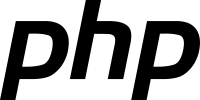
\includegraphics[width=1.5cm]{figures/diagram/php.png}};
\node[align = center, below = of ffr-api] [below=0.2cm of ffr-api]
	{\text\,FFR\\ API};

\node[inner sep=0pt] (acubed-database-sync) at (8,8)
    {
\includegraphics[width=1.5cm]{figures/diagram/github-actions.png}};
\node[align = center, below = of acubed-database-sync] [below=0.2cm of acubed-database-sync]
	{\text\,ACubed\\ Database Sync};

\node[inner sep=0pt] (acubed-database-reset) at (8,5)
    {
\includegraphics[width=1.5cm]{figures/diagram/github-actions.png}};
\node[align = center, below = of acubed-database-reset] [below=0.2cm of acubed-database-reset]
	{\text\,ACubed\\ Database Reset};

    \node[inner sep=0pt] (acubed-database) at (12,5)
    {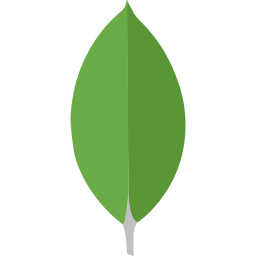
\includegraphics[width=1.5cm]{figures/diagram/mongodb.png}};
\node[align = center, below = of acubed-database] [below=0.2cm of acubed-database]
	{\text\,ACubed\\ Database};
    
    \node[inner sep=0pt] (acubed-codebase) at (12,-1.5)
    {
\includegraphics[width=1.5cm]{figures/diagram/python.png}};
\node[align = center, below = of acubed-codebase] [below=0.2cm of acubed-codebase]
	{\text\,ACubed\\ Codebase};

    \node[inner sep=0pt] (stepfile-difficulty-model) at (8,1.5)
    {
\includegraphics[width=1.5cm]{figures/diagram/difficulty-model.png}};
\node[align = center, below = of stepfile-difficulty-model] [below=0.2cm of stepfile-difficulty-model]
	{\text\,Stepfile Difficulty\\ Model};

    \node[inner sep=0pt] (aaa-equivalency-model) at (8,-1.5)
    {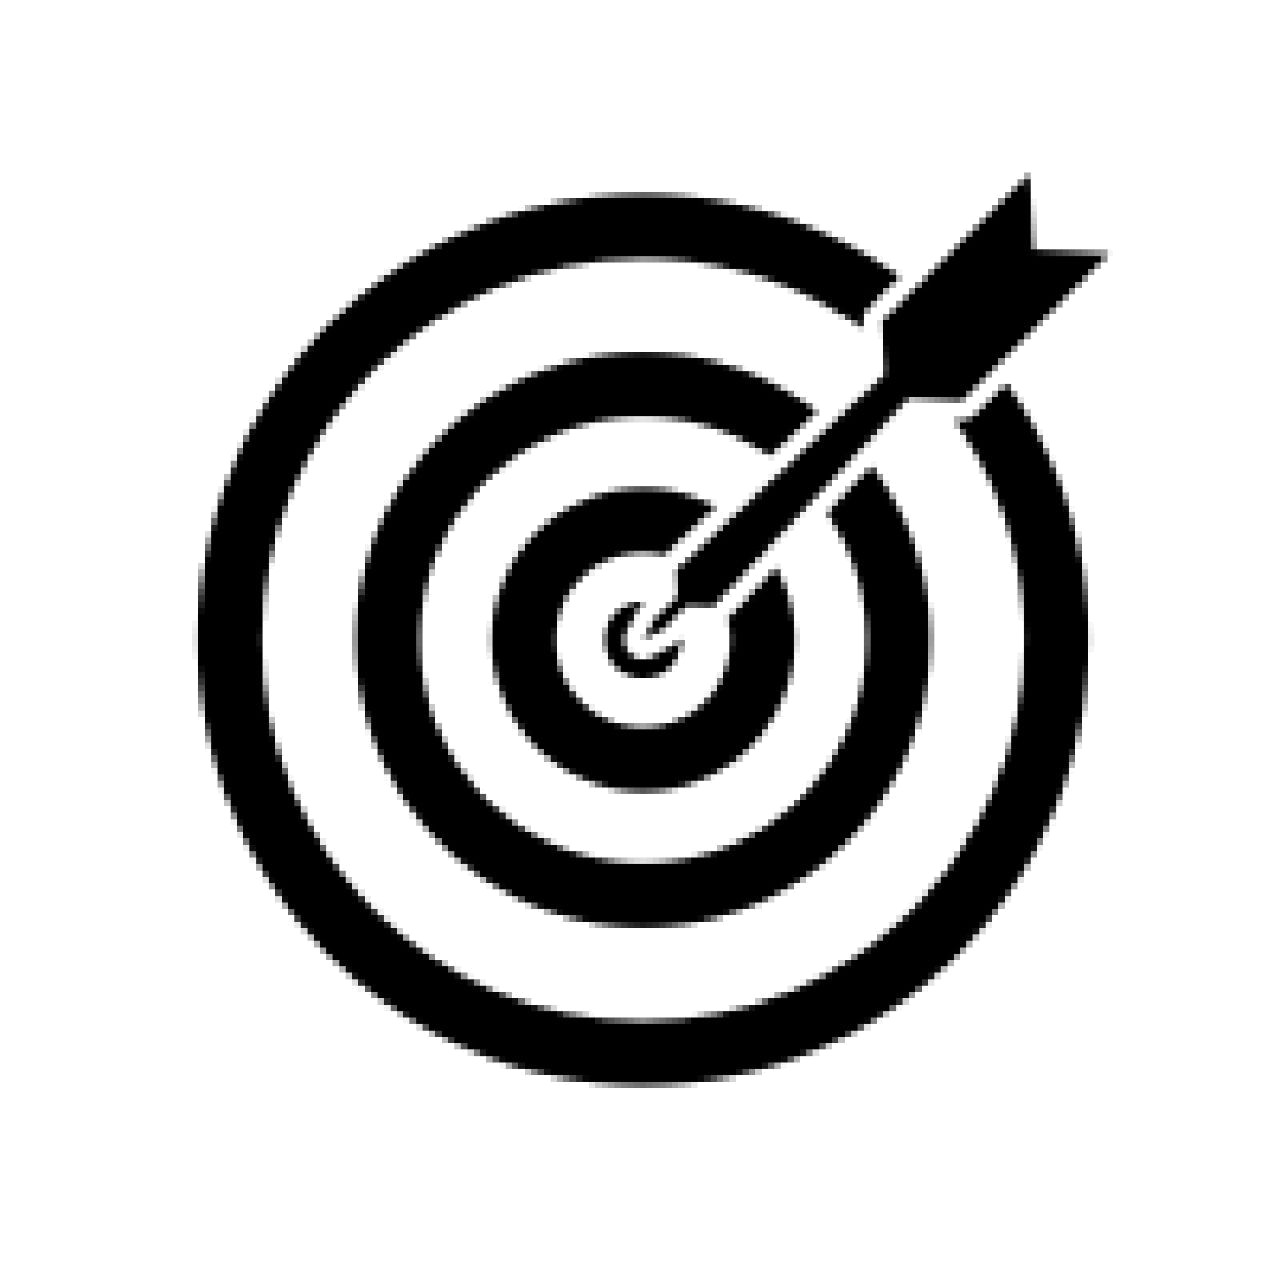
\includegraphics[width=1.5cm]{figures/diagram/aaa-equiv.png}};
\node[align = center, below = of aaa-equivalency-model] [below=0.2cm of aaa-equivalency-model]
	{\text\,AAA Equivalency\\ Model};

    \node[inner sep=0pt] (skill-rating-model) at (8,-4.5)
    {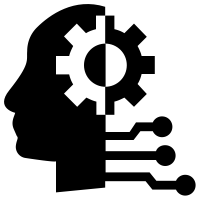
\includegraphics[width=1.5cm]{figures/diagram/skill-rating.png}};
\node[align = center, below = of skill-rating-model] [below=0.2cm of skill-rating-model]
	{\text\,Skill Rating\\ Model};

    \node[inner sep=0pt] (acubed-api) at (4,1.5)
    {
\includegraphics[width=1.5cm]{figures/diagram/fastapi.png}};
\node[align = center, below = of acubed-api] [below=0.2cm of acubed-api]
	{\text\,ACubed\\ API};

    \node[inner sep=0pt] (rcubed-codebase) at (4,-1.5)
    {
\includegraphics[width=1.5cm]{figures/diagram/rcubed.png}};
\node[align = center, below = of rcubed-codebase] [below=0.2cm of rcubed-codebase]
	{\text\,RCubed\\ Codebase};

    \node[inner sep=0pt] (ffr-engine) at (4,-8)
    {
\includegraphics[width=1.5cm]{figures/diagram/air.png}};
\node[align = center, below = of ffr-engine] [below=0.2cm of ffr-engine]
	{\text\,FFR\\ Engine};

    \node[inner sep=0pt] (ffr-website) at (8,-8)
    {
\includegraphics[width=1.5cm]{figures/diagram/website.png}};
\node[align = center, below = of ffr-website] [below=0.2cm of ffr-website]
	{\text\,FFR\\ Website};
    
% ffr-database to ffr-api
\draw[-,thick] (0, 2.5) -- (0,5);
\draw[->,thick] (0, 5) -- (3, 5);

% ffr-api to acubed-database-reset
\draw[->,dotted,thick] (5, 5) -- (7, 5);

% ffr-api to acubed-database-sync
\draw[-,thick] (4, 6) -- (4,8);
\draw[->,thick] (4, 8) -- (7, 8);

% acubed-database-sync to acubed-database
\draw[-,thick] (9, 8) -- (12, 8);
\draw[->,thick] (12, 8) -- (12,6);

% acubed-database-sync to acubed-database
\draw[->,dotted,thick] (9, 5) -- (11, 5);

% acubed-database to acubed-codebase
\draw[->,dotted,thick] (12, 3) -- (12, -0.5);

% acubed-codebase to models
\draw[-,dotted,thick] (11, -1.5) -- (10.5, -1.5);
\draw[-,dotted,thick] (10.5, -1.5) -- (10.5, 1.5);
\draw[-,dotted,thick] (10.5, -1.5) -- (10.5, -4.5);
\draw[->,dotted,thick] (10.5, 1.5) -- (9, 1.5);
\draw[->,dotted,thick] (10.5, -1.5) -- (9, -1.5);
\draw[->,dotted,thick] (10.5, -4.5) -- (9, -4.5);

% models to targets
\draw[->,thick] (7, 1.5) -- (5, 1.5);
\draw[->,thick] (7, -1.5) -- (5, -1.5);
\draw[->,thick] (8, -6.5) -- (8, -7);

% acubed-api to ffr-database
\draw[->,dotted,thick] (3, 1.5) -- (1, 1.5);

% ffr-database to ffr-codebase
\draw[-,thick] (0, -0.5) -- (0, -1.5);
\draw[->,thick] (0, -1.5) -- (3, -1.5);

% ffr-codebase to ffr-engine
\draw[->,thick] (4, -3.5) -- (4, -7);

% ffr-engine to ffr-website
\draw[->,thick] (5, -8) -- (7, -8);


\end{tikzpicture}
}
\end{center}

Lorem ipsum dolor sit amet, consectetur adipiscing elit. Etiam fermentum sapien a felis mattis fermentum. Nunc laoreet eros in malesuada ultricies. Sed purus libero, blandit vitae convallis eu, lacinia ut justo. Curabitur est mauris, tincidunt in lacinia et, varius nec tortor. Nunc eu turpis feugiat, porta diam non, tincidunt lorem. Sed pulvinar, metus a volutpat malesuada, urna quam tempor nisi, nec cursus urna dolor vitae felis. Pellentesque posuere neque sapien, quis sagittis neque luctus quis. Quisque ullamcorper dignissim suscipit. Maecenas pharetra, nisi a pretium placerat, ante est posuere mauris, nec auctor mi diam in nisl. Pellentesque ligula magna, volutpat sed nunc vitae, auctor gravida arcu. Maecenas sit amet lacus justo.

\vspace{2mm}

In eu finibus purus. Etiam accumsan erat justo, eu efficitur elit faucibus non. In faucibus vitae nisl dapibus ullamcorper. In fermentum leo eu purus rutrum suscipit. Pellentesque dictum efficitur purus, eu consequat metus pretium a. Vivamus feugiat urna ac accumsan suscipit. Praesent pretium sem risus, a congue felis placerat sed. Maecenas in nisi auctor, aliquet tortor ut, posuere justo. Cras lacinia bibendum elit, ut cursus turpis eleifend vitae. Nunc tempus libero quis suscipit scelerisque. Curabitur aliquet tempor facilisis. Suspendisse auctor, arcu non dictum luctus, sem tortor varius lorem, non commodo nibh arcu non elit. Maecenas maximus maximus justo, vitae bibendum orci semper eget.

\vspace{2mm}

Sed pulvinar leo eget nunc placerat, at cursus quam commodo. Vivamus nunc nisl, posuere id nunc ac, vehicula suscipit dui. Vivamus sodales urna felis, eget gravida nunc dignissim vel. Nam sed libero quis elit fermentum rhoncus. Vestibulum vitae libero et lectus ullamcorper congue eu in ex. In id ultricies enim. Integer volutpat nisi a lorem malesuada ultricies. Pellentesque ut commodo nulla. Nulla eu diam id lectus aliquet venenatis at quis ipsum.

\vspace{2mm}

Nulla ac mauris pharetra turpis interdum faucibus. Sed aliquam tellus ac finibus rutrum. Integer non vulputate sapien. Duis ullamcorper, felis non hendrerit interdum, ex lorem varius mauris, non consectetur eros tellus et ipsum. Nunc scelerisque turpis eu ullamcorper dictum. Cras ligula libero, pellentesque et pretium sed, tristique eget augue. Curabitur magna lectus, aliquam nec ullamcorper a, finibus pulvinar odio. Maecenas dictum, nisl et ornare porttitor, tortor metus molestie massa, ut porta nisi leo non velit. Maecenas quis rhoncus urna. Praesent a lacus vitae erat sagittis facilisis ac ac risus.

\vspace{2mm}

Quisque dapibus semper semper. Phasellus dignissim fringilla mollis. Duis volutpat lacus eget fringilla pretium. Phasellus ut orci non justo viverra aliquet sed at risus. Nulla eu tellus tincidunt, ultrices lectus vitae, tincidunt nibh. Vestibulum ante ipsum primis in faucibus orci luctus et ultrices posuere cubilia curae; Nullam sem orci, fringilla sed nisi et, rhoncus sollicitudin odio. Nam sodales tortor ante, sit amet porttitor ipsum cursus id. Maecenas dapibus mauris nunc, ut placerat dui volutpat vitae. Donec viverra nulla nec libero iaculis mollis. Nullam viverra sit amet felis eu condimentum. In et tempor nibh. Phasellus interdum nibh ornare, scelerisque elit ac, fringilla arcu. Nullam rutrum vestibulum sollicitudin. Proin sem ante, tincidunt et nisi et, ultricies vulputate purus.

\section{Conclusion and Acknowledgements}
\label{sec:conclusion}
Lorem ipsum dolor sit amet, consectetur adipiscing elit. Etiam fermentum sapien a felis mattis fermentum. Nunc laoreet eros in malesuada ultricies. Sed purus libero, blandit vitae convallis eu, lacinia ut justo. Curabitur est mauris, tincidunt in lacinia et, varius nec tortor. Nunc eu turpis feugiat, porta diam non, tincidunt lorem. Sed pulvinar, metus a volutpat malesuada, urna quam tempor nisi, nec cursus urna dolor vitae felis. Pellentesque posuere neque sapien, quis sagittis neque luctus quis. Quisque ullamcorper dignissim suscipit. Maecenas pharetra, nisi a pretium placerat, ante est posuere mauris, nec auctor mi diam in nisl. Pellentesque ligula magna, volutpat sed nunc vitae, auctor gravida arcu. Maecenas sit amet lacus justo.

\vspace{2mm}

In eu finibus purus. Etiam accumsan erat justo, eu efficitur elit faucibus non. In faucibus vitae nisl dapibus ullamcorper. In fermentum leo eu purus rutrum suscipit. Pellentesque dictum efficitur purus, eu consequat metus pretium a. Vivamus feugiat urna ac accumsan suscipit. Praesent pretium sem risus, a congue felis placerat sed. Maecenas in nisi auctor, aliquet tortor ut, posuere justo. Cras lacinia bibendum elit, ut cursus turpis eleifend vitae. Nunc tempus libero quis suscipit scelerisque. Curabitur aliquet tempor facilisis. Suspendisse auctor, arcu non dictum luctus, sem tortor varius lorem, non commodo nibh arcu non elit. Maecenas maximus maximus justo, vitae bibendum orci semper eget.

\vspace{2mm}

Sed pulvinar leo eget nunc placerat, at cursus quam commodo. Vivamus nunc nisl, posuere id nunc ac, vehicula suscipit dui. Vivamus sodales urna felis, eget gravida nunc dignissim vel. Nam sed libero quis elit fermentum rhoncus. Vestibulum vitae libero et lectus ullamcorper congue eu in ex. In id ultricies enim. Integer volutpat nisi a lorem malesuada ultricies. Pellentesque ut commodo nulla. Nulla eu diam id lectus aliquet venenatis at quis ipsum.

\vspace{2mm}

Nulla ac mauris pharetra turpis interdum faucibus. Sed aliquam tellus ac finibus rutrum. Integer non vulputate sapien. Duis ullamcorper, felis non hendrerit interdum, ex lorem varius mauris, non consectetur eros tellus et ipsum. Nunc scelerisque turpis eu ullamcorper dictum. Cras ligula libero, pellentesque et pretium sed, tristique eget augue. Curabitur magna lectus, aliquam nec ullamcorper a, finibus pulvinar odio. Maecenas dictum, nisl et ornare porttitor, tortor metus molestie massa, ut porta nisi leo non velit. Maecenas quis rhoncus urna. Praesent a lacus vitae erat sagittis facilisis ac ac risus.

\vspace{2mm}

Quisque dapibus semper semper. Phasellus dignissim fringilla mollis. Duis volutpat lacus eget fringilla pretium. Phasellus ut orci non justo viverra aliquet sed at risus. Nulla eu tellus tincidunt, ultrices lectus vitae, tincidunt nibh. Vestibulum ante ipsum primis in faucibus orci luctus et ultrices posuere cubilia curae; Nullam sem orci, fringilla sed nisi et, rhoncus sollicitudin odio. Nam sodales tortor ante, sit amet porttitor ipsum cursus id. Maecenas dapibus mauris nunc, ut placerat dui volutpat vitae. Donec viverra nulla nec libero iaculis mollis. Nullam viverra sit amet felis eu condimentum. In et tempor nibh. Phasellus interdum nibh ornare, scelerisque elit ac, fringilla arcu. Nullam rutrum vestibulum sollicitudin. Proin sem ante, tincidunt et nisi et, ultricies vulputate purus.

\clearpage

%----------------------------------------------------------------------------------------
%	Appendix
%----------------------------------------------------------------------------------------
\appendix

\section{Appendix}
\label{sec:appendix}
Lorem ipsum dolor sit amet, consectetur adipiscing elit. Etiam fermentum sapien a felis mattis fermentum. Nunc laoreet eros in malesuada ultricies. Sed purus libero, blandit vitae convallis eu, lacinia ut justo. Curabitur est mauris, tincidunt in lacinia et, varius nec tortor. Nunc eu turpis feugiat, porta diam non, tincidunt lorem. Sed pulvinar, metus a volutpat malesuada, urna quam tempor nisi, nec cursus urna dolor vitae felis. Pellentesque posuere neque sapien, quis sagittis neque luctus quis. Quisque ullamcorper dignissim suscipit. Maecenas pharetra, nisi a pretium placerat, ante est posuere mauris, nec auctor mi diam in nisl. Pellentesque ligula magna, volutpat sed nunc vitae, auctor gravida arcu. Maecenas sit amet lacus justo.

\vspace{2mm}

In eu finibus purus. Etiam accumsan erat justo, eu efficitur elit faucibus non. In faucibus vitae nisl dapibus ullamcorper. In fermentum leo eu purus rutrum suscipit. Pellentesque dictum efficitur purus, eu consequat metus pretium a. Vivamus feugiat urna ac accumsan suscipit. Praesent pretium sem risus, a congue felis placerat sed. Maecenas in nisi auctor, aliquet tortor ut, posuere justo. Cras lacinia bibendum elit, ut cursus turpis eleifend vitae. Nunc tempus libero quis suscipit scelerisque. Curabitur aliquet tempor facilisis. Suspendisse auctor, arcu non dictum luctus, sem tortor varius lorem, non commodo nibh arcu non elit. Maecenas maximus maximus justo, vitae bibendum orci semper eget.

\vspace{2mm}

Sed pulvinar leo eget nunc placerat, at cursus quam commodo. Vivamus nunc nisl, posuere id nunc ac, vehicula suscipit dui. Vivamus sodales urna felis, eget gravida nunc dignissim vel. Nam sed libero quis elit fermentum rhoncus. Vestibulum vitae libero et lectus ullamcorper congue eu in ex. In id ultricies enim. Integer volutpat nisi a lorem malesuada ultricies. Pellentesque ut commodo nulla. Nulla eu diam id lectus aliquet venenatis at quis ipsum.

\vspace{2mm}

Nulla ac mauris pharetra turpis interdum faucibus. Sed aliquam tellus ac finibus rutrum. Integer non vulputate sapien. Duis ullamcorper, felis non hendrerit interdum, ex lorem varius mauris, non consectetur eros tellus et ipsum. Nunc scelerisque turpis eu ullamcorper dictum. Cras ligula libero, pellentesque et pretium sed, tristique eget augue. Curabitur magna lectus, aliquam nec ullamcorper a, finibus pulvinar odio. Maecenas dictum, nisl et ornare porttitor, tortor metus molestie massa, ut porta nisi leo non velit. Maecenas quis rhoncus urna. Praesent a lacus vitae erat sagittis facilisis ac ac risus.

\vspace{2mm}

Quisque dapibus semper semper. Phasellus dignissim fringilla mollis. Duis volutpat lacus eget fringilla pretium. Phasellus ut orci non justo viverra aliquet sed at risus. Nulla eu tellus tincidunt, ultrices lectus vitae, tincidunt nibh. Vestibulum ante ipsum primis in faucibus orci luctus et ultrices posuere cubilia curae; Nullam sem orci, fringilla sed nisi et, rhoncus sollicitudin odio. Nam sodales tortor ante, sit amet porttitor ipsum cursus id. Maecenas dapibus mauris nunc, ut placerat dui volutpat vitae. Donec viverra nulla nec libero iaculis mollis. Nullam viverra sit amet felis eu condimentum. In et tempor nibh. Phasellus interdum nibh ornare, scelerisque elit ac, fringilla arcu. Nullam rutrum vestibulum sollicitudin. Proin sem ante, tincidunt et nisi et, ultricies vulputate purus.


%----------------------------------------------------------------------------------------
%	Bibliography
%----------------------------------------------------------------------------------------

\printbibliography

\end{document}